
\section{四个例子}\label{sec:11-3}

本节讨论 Fano \BookRecordIndex{T0169}环面流形、格拉斯曼流形和\BookRecordIndex{T0274}旗流形的\BookRecordIndex{T0229}量子上同调，并解释它们同 \BookRecordIndex{T0050}Toda
晶格及 Verlinde 代数的联系。所有这些流形都是 Fano 的，也就是说，对每个有全纯代表的
类 $A$，都有 $c_1(A)>0$（见注~\ref{rem:11-1-1}）。当这一条件不满足时，会出现新的
现象。这里我们用 Calabi--Yau 三维簇来说明这一点。另一个例子见第~\ref{sec:11-4} 节，
那里将描述非 Fano \BookRecordIndex{T0169}环面流形的\BookRecordIndex{T0229}量子上同调。在前三种情形，我们会给出\BookRecordIndex{T0229}量子上同调环的
表示。不过，正如注~\ref{rem:11-3-20} 所表明的，这甚至还不足以导出\BookRecordIndex{T0144}格罗莫夫--威滕势中
三次项的公式。在 Calabi--Yau 的例子中，这个势有一个最初由镜像对称得到的公式。

\subsection{Fano \BookRecordIndex{T0169}环面流形}\label{subsec:11-3-1}

本小节介绍 Batyrev \srcite{31} 最先给出的 Fano \BookRecordIndex{T0169}环面流形小\BookRecordIndex{T0229}量子上同调环公式。这个
公式在 Givental \srcite{150} 关于镜像对称的工作中起重要作用；他把它置于等变\BookRecordIndex{T0229}量子上
同调的框架中。下面简述 Cieliebak--Salamon \srcite{69} 基于\BookRecordIndex{T0356}辛涡旋方程的一种相当不同
的证明。McDuff--Tolman \srcite{279} 的另一个证明将在第~\ref{sec:11-4} 节中勾勒。
我们先描述\BookRecordIndex{T0169}环面流形的结构。虽然这需要一些工作，最终却会得到一族显式、易于掌握的
非平凡例子。更多资料可参见 Audin \srcite{23}、Cox--Katz \srcite{76}、
Guillemin--Sternberg \srcite{164} 或 Voisin \srcite{409}。

我们说明观察\BookRecordIndex{T0169}环面流形的两种方式。第一种是把它看成闭\BookRecordIndex{T0358}辛流形 $(M,\omega)$，其上带有
有效的哈密顿环面作用；环面的维数是 $M$ 维数的一半，而“有效”是指 $M$ 中存在一点，
环面在该点上的作用是自由的。第二种是把\BookRecordIndex{T0169}环面流形（或轨形）看成 $\mathbb C^N$ 上
线性环面作用在恰当\BookRecordIndex{T0204}矩映射下的辛商。要得到完整图景，须把两种观点结合起来。我们从
第二种开始。

设 $T$ 是 $k$ 维环面，以 $\mathfrak t$ 表示其李代数，并以
\[
  \Lambda:=\{\xi\in\mathfrak t\mid\exp(\xi)=1\}
\]
表示整数格，以
\[
  \Lambda^*:=\{w\in\mathfrak t^*\mid
  \langle w,\xi\rangle\in\mathbb Z\text{ 对所有 }\xi\in\Lambda\}
\]
表示对偶格。假设 $T$ 通过同态
\[
  \rho=\operatorname{diag}(\rho_1,\ldots,\rho_N):
  T\longrightarrow T^N\subset U(N)
\]
作用在 $\mathbb C^N$ 上；这里 $T^N$ 是 $U(N)$ 的对角子群。对
$\nu=1,\ldots,N$，把同态 $\rho_\nu:T\to S^1$ 写成
\begin{equation}\label{eq:11-3-1}
  \rho_\nu(\exp\xi)=e^{-2\pi i\langle w_\nu,\xi\rangle},
  \qquad \xi\in\mathfrak t,
\end{equation}
其中 $w_\nu\in\Lambda^*$。这个作用的一个\BookRecordIndex{T0204}矩映射
$\mu:\mathbb C^N\to\mathfrak t^*$ 为
\begin{equation}\label{eq:11-3-2}
  \mu(x):=\pi\sum_{\nu=1}^N|x_\nu|^2w_\nu.
\end{equation}
我们假设\BookRecordIndex{T0204}矩映射是恰当的，也就是说，$\mathfrak t^*$ 中存在一个包含所有 $w_\nu$ 的开半
空间。还假设作用有效，也就是说，向量 $w_\nu$ 张成 $\mathfrak t^*$ 中的整数格
$\Lambda^*$。

\BookRecordIndex{T0204}矩映射在\BookRecordIndex{T0409}正则值 $\tau\in\mathfrak t^*$ 处的辛商定义为\sourcefootnote{原书在此定义
及紧接着的复化商中把环境空间误印为 $\mathbb C^n$；但本段的作用、坐标和\BookRecordIndex{T0204}矩映射均定义在
$\mathbb C^N$ 上，故补正为 $\mathbb C^N$。}
\[
  M_\tau:=\mathbb C^N/\!/T(\tau):=\mu^{-1}(\tau)/T.
\]
当 $T$ 在 $\mu^{-1}(\tau)$ 上自由作用时，这个商是闭\BookRecordIndex{T0358}辛流形；否则它是闭辛轨形。商
$\mu^{-1}(\tau)/T$ 还可与 $U/T^{\mathbb C}$ 识别，其中 $U$ 是 $\mathbb C^N$ 的一个
适当开子集，而 $T^{\mathbb C}\cong(\mathbb C^*)^k$ 是实环面 $T$ 的复化。因此
$M_\tau$ 是 \BookRecordIndex{T0207}凯勒 流形，事实上是光滑射影簇，所以可按注~\ref{rem:11-1-1} 所讨论的
射影语境理解 Fano 一词。更多细节见上述文献或 McDuff--Tolman
\srcite{280, \S5}。

现在假设 $\tau$ 是 $\mu$ 的\BookRecordIndex{T0409}正则值，并且 $T$ 在 $\mu^{-1}(\tau)$ 上自由作用。对每个子集
$I\subset I_0:=\{1,\ldots,N\}$，考虑子空间
\[
  E_I:=\mathbb C^{I_0\setminus I}
  =\{x\in\mathbb C^N\mid x_\nu=0\text{ 对 }\nu\in I\},
\]
并以
\[
  \operatorname{cone}(I):=
  \left\{\sum_{\nu\in I}\eta_\nu w_\nu\,\middle|\,
  \eta_\nu\geq0\right\}\subset\mathfrak t^*
\]
表示由 $\{w_\nu\}_{\nu\in I}$ 张成的闭正锥。由式~\eqref{eq:11-3-2}，
\begin{equation}\label{eq:11-3-3}
  E_I\cap\mu^{-1}(\tau)\ne\varnothing
  \quad\Longleftrightarrow\quad
  \tau\in\operatorname{cone}(I_0\setminus I).
\end{equation}
相应的 $M_\tau$ 子流形
\begin{equation}\label{eq:11-3-4}
  X_I:=\bigl(E_I\cap\mu^{-1}(\tau)\bigr)/T
  =\{[x]\in M_\tau\mid x_\nu=0\text{ 对 }\nu\in I\}
\end{equation}
在如下意义下生成其上同调。若 $I=\{\nu\}$ 是单点集，则
\[
  X_\nu:=\{[x]\in M_\tau\mid x_\nu=0\}
\]
是光滑除子（即复余维一的子流形），并确定上同调类
$\overline w_\nu:=\operatorname{PD}([X_\nu])\in H^2(M_\tau)$。因此
$\overline w_\nu$ 是线丛
\begin{equation}\label{eq:11-3-5}
  L_\nu:=\mu^{-1}(\tau)\times_{\rho_\nu}\mathbb C\longrightarrow M_\tau
\end{equation}
的第一 Chern 类。注意，$\overline w_\nu=0$ 当且仅当 $X_\nu=\varnothing$，这恰发生在
$\tau\notin\operatorname{cone}(I_0\setminus\{\nu\})$ 时。此外，
$X_{I\cup I'}=X_I\cap X_{I'}$。
\sourcefootnote{原书把左端下标的并集误印为 $I\cap I'$；由
$X_I=\{[x]\mid x_\nu=0\text{ 对 }\nu\in I\}$ 的定义，两个零坐标条件的交集对应
指标集的并集，紧接着的 $X_{\{\nu_1,\ldots,\nu_k\}}$ 也印证了这一点。}
所以
\[
  X_{\{\nu_1,\ldots,\nu_k\}}=\varnothing
  \quad\Longrightarrow\quad
  \overline w_{\nu_1}\smile\cdots\smile\overline w_{\nu_k}=0.
\]
由式~\eqref{eq:11-3-5}，表示 $\rho_\nu$ 之间的每个关系
$\sum_\nu\eta_\nu w_\nu=0$ 都在上同调类之间给出相应关系
$\sum_\nu\eta_\nu\overline w_\nu=0$。事实证明，这些就是 $\overline w_\nu$ 之间的全部
关系。下述定理的证明见 Guillemin--Sternberg \srcite{164}。

\begin{theorem}\label{thm:11-3-1}
设 $\tau\in\mathfrak t^*$ 是 $\mu$ 的\BookRecordIndex{T0409}正则值，并假设 $T$ 在 $\mu^{-1}(\tau)$ 上自由作用。
则环同态
\[
  \mathbb R[u_1,\ldots,u_N]\longrightarrow H^*(M_\tau;\mathbb R),
  \qquad u_\nu\longmapsto\overline w_\nu
\]
诱导同构
\[
  H^*(M_\tau;\mathbb R)\cong\mathbb R[u_1,\ldots,u_N]/\mathcal I,
\]
其中理想 $\mathcal I\subset\mathbb R[u_1,\ldots,u_N]$ 由下列关系生成：
\begin{align}
  \sum_{\nu=1}^N\eta_\nu w_\nu=0
  &\quad\Longrightarrow\quad
  \sum_{\nu=1}^N\eta_\nu u_\nu=0,
  \label{eq:11-3-6}\\
  I\subset I_0,\quad
  \tau\notin\operatorname{cone}(I_0\setminus I)
  &\quad\Longrightarrow\quad
  \prod_{\nu\in I}u_\nu=0.
  \label{eq:11-3-7}
\end{align}
\end{theorem}

\begin{remark}\label{rem:11-3-2}
设 $\tau\in\mathfrak t^*$ 是 $\mu$ 的\BookRecordIndex{T0409}正则值。则 $T$ 在 $\mu^{-1}(\tau)$ 上自由作用，当且
仅当下述整性条件成立：对每个恰有 $k$ 个元素且满足
$\tau\in\operatorname{cone}(J)$ 的子集 $J\subset I_0$，向量
$\{w_\nu\mid\nu\in J\}$ 构成整数格 $\Lambda^*$ 的一组基。此外可以证明，
$TM_\tau$ 的第一 Chern 类以及\BookRecordIndex{T0363}辛形式
$\omega_\tau\in\Omega^2(M_\tau)$ 的上同调类分别为
\[
  c_1(M_\tau)=\overline w_1+\cdots+\overline w_N,
  \qquad [\omega_\tau]=\overline\tau,
\]
其中 $\overline\tau$ 是 $\tau\in\mathfrak t^*$ 在由式~\eqref{eq:11-3-1} 和
\eqref{eq:11-3-5} 构造的同态
\[
  \mathfrak t^*=\Lambda^*\otimes\mathbb R
  \longrightarrow H^2(M_\tau;\mathbb R),\qquad w\longmapsto\overline w
\]
下的像。因此，$M_\tau$ 单调当且仅当 $\tau$ 是向量
$w_1+\cdots+w_N$ 的正倍数。（更多细节见 Cieliebak--Salamon
\srcite{69, Appendix C}。）
\end{remark}

\begin{example}\label{ex:11-3-3}
这个构造最简单的情形是 $k=1$。此时每个正的 $\tau\in\mathfrak t^*\cong\mathbb R$ 都是
\BookRecordIndex{T0409}正则值，而 $\mu^{-1}(\tau)$ 是球面 $S^{2N-1}$。恰当性条件意味着，对
$i=1,\ldots,N$，每个权 $w_i$ 都是 $\Lambda^*=\mathbb Z$ 的一个选定生成元 $w$ 的
正整数倍 $a_iw$。所得商称为加权射影空间。

只要 $I\ne\varnothing$，每个非零的 $\tau\in\mathfrak t^*$ 都属于
$\operatorname{cone}(I)$。因而注~\ref{rem:11-3-2} 表明，只有当所有 $a_i=1$ 时，
$S^1$ 才在 $\mu^{-1}(\tau)$ 上自由作用。在这种情形，$T=S^1$ 在 $\mathbb C^N$ 上按
对角方式作用，商就是标准射影空间 $\mathbb{CP}^{N-1}$。定理~\ref{thm:11-3-1} 把它的
上同调环表示为 $\mathbb R[u_1,\ldots,u_N]/\mathcal I$，其中 $\mathcal I$ 由关系
\[
  u_1=\cdots=u_N,\qquad \prod_{i=1}^N u_i=0
\]
生成。注意，只有一个乘法关系，对应于 $I=I_0$；事实上，若 $I\ne I_0$，则
$\operatorname{cone}(I_0\setminus I)=[0,\infty)$，因而包含 $\tau$。
\sourcefootnote{原书最后一句把锥误写为 $\operatorname{cone}(I\setminus I_0)$；但
式~\eqref{eq:11-3-3}--\eqref{eq:11-3-7} 中始终出现的是 $I_0\setminus I$。原句的条件
$I\ne I_0$ 也须保留：这正说明除 $I=I_0$ 外不会产生乘法关系。}
\end{example}

以上用 $\mathfrak t^*$ 中的元素 $w_1,\ldots,w_N$ 与 $\tau$ 描述了 $M_\tau$ 的结构。
下面说明，这一描述可完全改写为商 $M_\tau$ 上 $T^N/\rho(T)$ 作用的矩多面体 $\Delta$
的语言；比较例~\ref{ex:11-3-7}。

定理~\ref{thm:11-3-1} 表明，$H^2(M_\tau)$ 是 $\mathfrak t^*$ 中整数格的一个商。因此其
对偶 $H_2(M_\tau)$ 可与 $\Lambda\subset\mathfrak t$ 的如下子格识别：
\[
  \Lambda(\tau):=\left\{\lambda\in\Lambda\,\middle|\,
  \tau\notin\operatorname{cone}(I_0\setminus\{\nu\})
  \Longrightarrow\langle w_\nu,\lambda\rangle=0\right\}.
\]
在许多情形，对所有 $\nu$ 都有
$\tau\in\operatorname{cone}(I_0\setminus\{\nu\})$（这是一个非退化条件），于是
$\Lambda(\tau)$ 就等于 $\mathfrak t$ 中的整数格 $\Lambda$。一般而言，它的维数为
$m\leq k$。

以 $C(\tau)\subset\mathfrak t^*$ 表示\BookRecordIndex{T0204}矩映射 $\mu$ 的\BookRecordIndex{T0409}正则值集合中包含 $\tau$ 的连通分支。
这个集合称为 $\tau$ 的\BookRecordIndex{T0280}腔；它是 $\mathfrak t^*$ 中的开凸锥，也称为 $M_\tau$ 的 凯勒
锥。整数格 $\Lambda(\tau)$ 中的对偶锥，是由所有满足如下条件的
$\lambda\in\Lambda(\tau)$ 组成的闭凸锥：对每个 $\tau'\in C(\tau)$，都有
$\langle\tau',\lambda\rangle\geq0$。当 $\lambda\ne0$ 时，由于 $C(\tau)$ 是开的，这一条件
等价于对每个 $\tau'\in C(\tau)$ 都有 $\langle\tau',\lambda\rangle>0$。文献
\srcite{76, 69} 证明，这个对偶锥由有效类生成，即由能被（可能为常值的）全纯曲线表示的
类生成。记作\footnote{第~\ref{sec:11-1} 节为
\BookRecordIndex{T0207}凯勒流形 $(M,\omega,J)$ 定义了两种\BookRecordIndex{T0390}有效锥：由具有
非平凡\BookRecordIndex{T0143}格罗莫夫--威滕不变量的类生成的\BookRecordIndex{T0367}辛锥 $K^{\mathrm{eff}}(M,\omega)$，以及由全纯曲线
所表示的类生成的代数锥 $K^{\mathrm{eff}}(M,J)$。因此
$\Lambda^{\mathrm{eff}}(\tau):=K^{\mathrm{eff}}(M_\tau,J)$。在 Fano 情形，
定理~\ref{thm:11-3-4} 蕴含这两个锥相同：式~\eqref{eq:11-3-10} 表明，对每个非零的
$\lambda\in\Lambda^{\mathrm{eff}}(\tau)$，都有某个\BookRecordIndex{T0143}格罗莫夫--威滕不变量
$\operatorname{GW}_{\lambda,k}\ne0$。不过，在证明它之前，我们只知道 \BookRecordIndex{T0207}凯勒 流形 $(M,\omega,J)$ 定义了两种\BookRecordIndex{T0390}有效锥：由具有
非平凡\BookRecordIndex{T0143}格罗莫夫--威滕不变量的类生成的\BookRecordIndex{T0367}辛锥 $K^{\mathrm{eff}}(M,\omega)$，以及由全纯曲线
所表示的类生成的代数锥 $K^{\mathrm{eff}}(M,J)$。因此
$\Lambda^{\mathrm{eff}}(\tau):=K^{\mathrm{eff}}(M_\tau,J)$。在 Fano 情形，
定理~\ref{thm:11-3-4} 蕴含这两个锥相同：式~\eqref{eq:11-3-10} 表明，对每个非零的
$\lambda\in\Lambda^{\mathrm{eff}}(\tau)$，都有某个\BookRecordIndex{T0143}格罗莫夫--威滕不变量
$\operatorname{GW}_{\lambda,k}\ne0$。不过，在证明它之前，我们只知道
$K^{\mathrm{eff}}(M,\omega)\subset K^{\mathrm{eff}}(M,J)$。}
\[
  \Lambda^{\mathrm{eff}}(\tau):=
  \{\lambda\in\Lambda(\tau)\mid
  \tau'\in C(\tau)\Longrightarrow\langle\tau',\lambda\rangle\geq0\}.
\]

由此，$M_\tau$ 为 Fano 当且仅当向量
$c:=\sum_{\nu=1}^Nw_\nu$ 在 $\Lambda^{\mathrm{eff}}(\tau)\setminus\{0\}$ 上取正值。等价地，
$c$ 属于\BookRecordIndex{T0280}腔 $C(\tau)$；所以不妨假设 $c=\tau$，即 $M_\tau$ 单调。

以下假设 Fano \BookRecordIndex{T0169}环面流形上的\BookRecordIndex{T0363}辛形式 $\tau$ 选得使 $M_\tau$ 单调。固定
$\Lambda(\tau)$ 的一组整数基 $v_1,\ldots,v_m$，使每个
$\langle\tau,v_i\rangle>0$，且 $\Lambda^{\mathrm{eff}}(\tau)$ 的每个元素都是 $v_i$ 的
非负线性组合。再像例~\ref{ex:11-1-4}（iii）那样，取多项式环
$\mathbb R[q_1,\ldots,q_m]$ 为\BookRecordIndex{T0231}量子系数环。对满足 $\ell_\nu\geq0$ 的整数向量
$\ell=(\ell_1,\ldots,\ell_N)$，记
\[
  \overline w^{*\ell}:=
  (\underbrace{\overline w_1*\cdots*\overline w_1}_{\ell_1\text{ 次}})*\cdots*
  (\underbrace{\overline w_N*\cdots*\overline w_N}_{\ell_N\text{ 次}})
  \in QH^*(M_\tau;\mathbb R[q_1,\ldots,q_m]).
\]
下一个定理给出单调\BookRecordIndex{T0169}环面流形的 Batyrev \BookRecordIndex{T0229}量子上同调公式。注意，第一类关系正是
定理~\ref{thm:11-3-1} 所述普通上同调环中的关系。

\begin{theorem}[Batyrev、Givental、Cieliebak--Salamon]\label{thm:11-3-4}
设
\[
  \tau:=\sum_{\nu=1}^Nw_\nu
\]
是 $\mu$ 的\BookRecordIndex{T0409}正则值，并假设 $T$ 在 $\mu^{-1}(\tau)$ 上自由作用。则环同态
\[
  \mathbb R[u_1,\ldots,u_N,q_1,\ldots,q_m]
  \longrightarrow QH^*(M_\tau;\mathbb R[q_1,\ldots,q_m]),
  \qquad u^\ell\longmapsto\overline w^{*\ell}
\]
诱导同构
\[
  QH^*(M_\tau;\mathbb R[q_1,\ldots,q_m])
  \cong
  \mathbb R[u_1,\ldots,u_N,q_1,\ldots,q_m]/\mathcal J,
\]
其中理想 $\mathcal J$ 由下列关系生成：
\begin{align}
  \sum_{\nu=1}^N\eta_\nu w_\nu=0
  &\quad\Longrightarrow\quad
  \sum_{\nu=1}^N\eta_\nu u_\nu=0,
  \label{eq:11-3-8}\\
  \tau\notin\operatorname{cone}(I_0\setminus\{\nu\})
  &\quad\Longrightarrow\quad u_\nu=0,
  \label{eq:11-3-9}\\
  \lambda\in\Lambda^{\mathrm{eff}}(\tau),\quad
  d_\nu^\pm:=\max\{\pm\langle w_\nu,\lambda\rangle,0\}
  &\quad\Longrightarrow\quad u^{d^+}=q^\lambda u^{d^-}.
  \label{eq:11-3-10}
\end{align}
这里，若 $\lambda=\sum_i\lambda_iv_i\in\Lambda(\tau)$，则
$q^\lambda:=q_1^{\lambda_1}\cdots q_m^{\lambda_m}$。
\end{theorem}

下面的习题解释，最后的关系~\eqref{eq:11-3-10} 为什么是普通上同调中乘积关系的形变。

\begin{exercise}\label{ex:11-3-5}
给定 $\lambda\in\Lambda^{\mathrm{eff}}(\tau)$，令
$I:=\{\nu\mid\langle w_\nu,\lambda\rangle>0\}$。证明
$\tau\notin\operatorname{cone}(I_0\setminus I)$，并\BookRecordIndex{T0326}推出
$\overline w^{d^+}=0$ 在 $H^*(M_\tau)$ 中成立。
\end{exercise}

Cieliebak 和 Salamon 在 \srcite{69, Theorem C} 中给出的定理证明，还要附加假设
$M_\tau$ 的\BookRecordIndex{T0418}最小陈数至少为二。证明基于\BookRecordIndex{T0356}辛涡旋方程的性质。正如第~12.7 节将更详细
说明的，这些方程的解，是带哈密顿群作用之\BookRecordIndex{T0358}辛流形上的 \BookRecordIndex{T0003}$J$-全纯曲线的类似物。在这里，
辛涡旋\BookRecordIndex{T0246}模空间是紧的，而且可以通过\BookRecordIndex{T0078}穿墙公式计算不变量。Gaio--Salamon \srcite{135} 的
一个结果允许在单调情形比较涡旋不变量与商 $M_\tau$ 的\BookRecordIndex{T0143}格罗莫夫--威滕不变量。于是得到
如下形式的关系：
\[
  \operatorname{GW}_{A}^{M_\tau}(\overline w^{*d^+},a)
  =\operatorname{GW}_{A-A_\lambda}^{M_\tau}(\overline w^{*d^-},a),
\]
其中 $\lambda$ 与 $d^\pm$ 如式~\eqref{eq:11-3-10}，而
$A_\lambda\in H_2(M_\tau)$ 是同构
$\Lambda(\tau)\cong H_2(M_\tau)$ 下与 $\lambda\in\Lambda(\tau)$ 对应的同调类。这些关系
等价于~\eqref{eq:11-3-10}。若令 $q_i=0$，定理~\ref{thm:11-3-4} 中的理想
$\mathcal J$ 就等于定理~\ref{thm:11-3-1} 中的理想 $\mathcal I$；\BookRecordIndex{T0229}量子上同调具有所述形式
便由此得出。习题~\ref{ex:11-3-5} 表明 $\mathcal I$ 包含在 $\mathcal J$ 的像中；相等性
的证明见 Batyrev \srcite{31} 或 \srcite{69, Theorem C.5}。这些关系还有一种矩多面体
语言的解释，见下式~\eqref{eq:11-3-16}。定理~\ref{thm:11-3-4} 的另一种证明基于圆周作用
的 \BookRecordIndex{T0047}Seidel 表示，将在第~\ref{sec:11-4} 节末勾勒。

现在转向\BookRecordIndex{T0169}环面流形的第二种描述：它是一个闭\BookRecordIndex{T0358}辛流形 $(\overline M,\overline\omega)$，
其上有一个维数为 $\dim\overline M/2$ 的环面作有效哈密顿作用。以 $\overline T$ 表示这个
环面，以 $\overline{\mathfrak t}$ 表示其李代数。这个作用由一个
$\overline T$-不变\BookRecordIndex{T0204}矩映射
\[
  \overline\mu:\overline M\longrightarrow\overline{\mathfrak t}^{\,*}
\]
生成；这里，$\overline{\mathfrak t}$ 中元素 $\xi$ 的无穷小作用
$X_\xi\in\operatorname{Vect}(\overline M)$，是哈密顿函数
$H_\xi:=\langle\overline\mu,\xi\rangle$ 的\BookRecordIndex{T0160}哈密顿向量场，即
\[
  \iota(X_\xi)\overline\omega=dH_\xi,
  \qquad H_\xi:=\langle\overline\mu,\xi\rangle.
\]
Guillemin--Sternberg 与 Atiyah 的一个著名结果断言，\BookRecordIndex{T0204}矩映射的像
\[
  \Delta:=\overline\mu(\overline M)\subset\overline{\mathfrak t}^{\,*}
\]
是凸多面体。若 $\eta\in\Delta$ 位于一个 $k$ 维面的内部，则其逆像
$\overline\mu^{-1}(\eta)$ 是 $\overline T$ 的一个 $k$ 维轨道，而且必为各向同性的。特别地，
边（一维面）的逆像是二维球面。把 $\Delta$ 的余维一面
$F_1,\ldots,F_K$ 称为面片。每个面片 $F_\nu$ 都由如下形式的方程给出：
\[
  \{\eta\in\overline{\mathfrak t}^{\,*}\mid
    \langle\eta,\overline e_\nu\rangle=\kappa_\nu\},
\]
其中 $\kappa_\nu\in\mathbb R$ 称为结构常数，而
$\overline e_\nu\in\overline{\mathfrak t}$ 是整数格中的本原向量，称为
$F_\nu$ 的法向量。我们把法向量选成向内的，于是
\[
  \Delta=\overline\mu(\overline M)
  =\{\eta\in\overline{\mathfrak t}^{\,*}\mid
  \langle\eta,\overline e_\nu\rangle\geq\kappa_\nu,
  \ \nu=1,\ldots,K\}.
\]

Delzant \srcite{79} 证明，凸多面体 $\Delta$ 是某个\BookRecordIndex{T0169}环面流形的\BookRecordIndex{T0204}矩映射像，当且仅当
$\Delta$ 的每个顶点都满足：该顶点恰在 $n:=\dim\overline T$ 个面片上，而且相应的 $n$
个法向量构成 $\overline{\mathfrak t}$ 中整数格的一组基。由此可以把\BookRecordIndex{T0169}环面流形
$\overline M$ 构造成上述商 $M_\tau$。这里不作证明，不过，从下面关于两个构造之关系的
讨论中可以提取出一个证明。另见 Audin \srcite{23} 或 \srcite{280, \S5}。

在 $\overline M=M_\tau$ 的情形，商环面
\[
  \overline T:=T^N/\rho(T)
\]
作用在 $\overline M$ 上。其李代数是商
$\overline{\mathfrak t}:=\mathbb R^N/\dot\rho(\mathfrak t)$，其中诱导的李代数同态
$\dot\rho:\mathfrak t\to\mathbb R^N$ 由
$\dot\rho_\nu(\xi)=\langle w_\nu,\xi\rangle$ 给出；比较式~\eqref{eq:11-3-1}。
$\overline{\mathfrak t}$ 的对偶可与子空间
\begin{equation}\label{eq:11-3-11}
  \overline{\mathfrak t}^{\,*}:=
  \left\{\eta\in(\mathbb R^N)^*\,\middle|\,
  \sum_{\nu=1}^N\eta_\nu w_\nu=0\right\}
\end{equation}
识别。因此有正合列
\[
  0\longrightarrow\mathfrak t\xrightarrow{\dot\rho}\mathbb R^N
  \longrightarrow\overline{\mathfrak t}\longrightarrow0,
  \qquad
  0\longrightarrow\overline{\mathfrak t}^{\,*}\longrightarrow(\mathbb R^N)^*
  \longrightarrow\mathfrak t^*\longrightarrow0.
\]
法向量 $\overline e_\nu$ 属于 $\overline{\mathfrak t}$，而 $\tau,w_\nu$ 属于
$\mathfrak t^*$。还要注意，$\mathbb R^N$ 的标准基投影到法向量
$\overline e_\nu$，而 $(\mathbb R^N)^*$ 的标准基投影到重数向量 $w_\nu$。选取
$-\tau\in\mathfrak t^*$ 的一个提升
$\kappa=(\kappa_1,\ldots,\kappa_N)\in(\mathbb R^N)^*$，使
\[
  \sum_{\nu=1}^N\kappa_\nu w_\nu=-\tau\in\mathfrak t^*.
\]
于是能级集是\sourcefootnote{原书把这个能级条件误印成逐坐标等式
$\pi|x_\nu|^2=-\kappa_\nu$。由
$\mu(x)=\pi\sum_\nu|x_\nu|^2w_\nu=\tau$ 与
$\sum_\nu\kappa_\nu w_\nu=-\tau$，正确且等价的条件是向量
$(\pi|x_\nu|^2+\kappa_\nu)_\nu$ 位于式~\eqref{eq:11-3-11} 的核中；原条件还会使紧接着
定义的 $\overline\mu$ 恒为零。}
\[
  \mu^{-1}(\tau)=
  \left\{x\in\mathbb C^N\,\middle|\,
  (\pi|x_1|^2+\kappa_1,\ldots,\pi|x_N|^2+\kappa_N)
  \in\overline{\mathfrak t}^{\,*}\right\}.
\]
若以
\[
  [x]\in\overline M=\mu^{-1}(\tau)/T
\]
表示 $x\in\mu^{-1}(\tau)\subset\mathbb C^N$ 的 $T$-轨道，则式~\eqref{eq:11-3-2}
表明
\[
  \overline\mu:\overline M\longrightarrow\overline{\mathfrak t}^{\,*},
  \qquad
  [x]\longmapsto
  (\pi|x_1|^2+\kappa_1,\ldots,\pi|x_N|^2+\kappa_N)
\]
是一个\BookRecordIndex{T0204}矩映射。其像是凸多面体
\[
  \Delta=\overline\mu(\overline M)
  =\left\{\eta\in(\mathbb R^N)^*\,\middle|\,
  \sum_{\nu=1}^N\eta_\nu w_\nu=0,
  \ \eta_\nu\geq\kappa_\nu\right\}
  \subset\overline{\mathfrak t}^{\,*}.
\]
每个子集 $I\subset I_0:=\{1,\ldots,N\}$ 确定一个（可能为空的）面
\[
  \Delta_I:=\{\eta\in\Delta\mid\eta_\nu=\kappa_\nu
  \text{ 对 }\nu\in I\}.
\]
于是 $\Delta_\varnothing=\Delta$，并由式~\eqref{eq:11-3-3} 得
\begin{equation}\label{eq:11-3-12}
  \Delta_I\ne\varnothing
  \quad\Longleftrightarrow\quad
  \tau\in\operatorname{cone}(I_0\setminus I).
\end{equation}
特别地，矩多面体 $\Delta$ 的面片数 $K$，等于满足
$\tau\in\operatorname{cone}(I_0\setminus\{\nu\})$ 的指标 $\nu\in I_0$ 的个数。为简单
起见，以下假设每个 $\nu$ 都满足这一条件，\footnote{如果从商 $M$ 出发，总可以选择环面
$T$ 和同态 $\rho:T\to T^N$，使这一条件成立。不过，有时把 $M$ 表示成某个 $M_\tau$
而允许一些 $F_\nu$ 为空会很有用；这些空面片称为\BookRecordIndex{T0383}幽灵面片。}从而每个
$F_\nu=\Delta_\nu\ne\varnothing$。这个条件还蕴含 $\Lambda=\Lambda(\tau)$ 与 $m=k$。
注意，对所有 $I$，$\Delta_I$ 都是 $\nu\in I$ 对应的面片 $\Delta_\nu$ 的交。此外，
$F_\nu$ 的法向量 $\overline e_\nu$，就是 $\mathbb R^N$ 的标准基向量在商
$\overline{\mathfrak t}=\mathbb R^N/\dot\rho(\mathfrak t)$ 中的投影。

\begin{example}\label{ex:11-3-6}
像例~\ref{ex:11-3-3} 那样，把 $\mathbb{CP}^2$ 看成
$S^5=\mu^{-1}(1)$ 关于 $S^1$ 对角作用的商。此时所有权向量都是
$w_\nu=1\in\mathfrak t^*\cong\mathbb R$，所以矩多面体包含在超平面
$\{\sum_{\nu=1}^3\eta_\nu=0\}\subset\mathbb R^3$ 中，而 $\kappa$ 满足
$\sum_\nu\kappa_\nu=-1$。假设通过投影到前两个坐标，把商
$\overline{\mathfrak t}=\mathbb R^3/\mathfrak t$ 与 $\mathbb R^2$ 识别。由于三个法向量
$\overline e_\nu$ 是标准基的像，便有
\[
  \overline e_1=(1,0),\qquad
  \overline e_2=(0,1),\qquad
  \overline e_3=(-1,-1).
\]
相应的嵌入
$\mathbb R^2\cong\overline{\mathfrak t}^{\,*}\to
\{\sum_{\nu=1}^3\eta_\nu=0\}\subset\mathbb R^3$ 为
$(\xi_1,\xi_2)\mapsto(\xi_1,\xi_2,-\xi_1-\xi_2)$。因此，由于
$-\kappa_3=1+\kappa_1+\kappa_2$，矩多面体在 $\mathbb R^2$ 中的像是三角形\sourcefootnote{原书在三角形的第三个不等式中误把 $\xi_1+\xi_2$ 印成
$\xi_1\xi_2$；由第三坐标
$-\xi_1-\xi_2\geq\kappa_3$ 唯一得到这里的和式。}
\[
  \Delta_\kappa:=\{(\xi_1,\xi_2)\mid
  \xi_1\geq\kappa_1,\ \xi_2\geq\kappa_2,\
  \xi_1+\xi_2\leq1+\kappa_1+\kappa_2\}.
\]
改变 $-\tau=-1$ 的提升 $\kappa$ 对应于平移多面体，而改变
$\overline{\mathfrak t}$ 与 $\mathbb R^2$ 的识别，则以整仿射变换改变它。（总把这一识别
选成使 $\overline{\mathfrak t}$ 的整数格为 $\mathbb Z^2\subset\mathbb R^2$。）
\end{example}

式~\eqref{eq:11-3-4} 中的辛子流形 $X_\nu$ 现在由
\[
  X_\nu:=\overline\mu^{-1}(\Delta_\nu)
\]
给出，而上同调类 $\overline w_\nu$ 定义为它的庞加莱对偶。由
式~\eqref{eq:11-3-11}，关系~\eqref{eq:11-3-6} 改写为：对每个
$\eta\in\overline{\mathfrak t}^{\,*}$，
$\sum_\nu\langle\eta,\overline e_\nu\rangle\overline w_\nu=0$。另一方面，关系
~\eqref{eq:11-3-9} 是冗余的，因为每个 $\Delta_\nu\ne\varnothing$。
\sourcefootnote{原书把这里的回指标号误印为 (11.3.7)。关系 (11.3.7) 是下式仍保留的
Stanley--Reisner 乘积关系；而 $\Delta_\nu\ne\varnothing$ 恰使单指标关系 (11.3.9)
不产生任何 $u_\nu=0$ 关系。}
在这种记号下，
定理~\ref{thm:11-3-1} 断言
\[
  H^*(\overline M;\mathbb R)\cong
  \frac{\mathbb R[u_1,\ldots,u_N]}{P(\Delta)+SR(\Delta)},
\]
其中 $P(\Delta)$ 与 $SR(\Delta)$ 是 $\mathbb R[u_1,\ldots,u_N]$ 中的理想：
\[
  P(\Delta):=
  \left\langle\sum_\nu\langle\eta,\overline e_\nu\rangle u_\nu
  \mathrel{\Big|}\eta\in\overline{\mathfrak t}^{\,*}\right\rangle,
  \qquad
  SR(\Delta):=
  \left\langle\prod_{\nu\in I}u_\nu
  \mathrel{\Big|}\Delta_I=\varnothing\right\rangle.
\]
理想 $SR(\Delta)$ 称为 Stanley--Reisner 理想。它由所有如下\BookRecordIndex{T0060}本原子集
$I\subset\{1,\ldots,N\}$ 生成：$\Delta_I=\varnothing$，但对每个真子集
$I'\subsetneq I$ 都有 $\Delta_{I'}\ne\varnothing$。同上可得
\begin{equation}\label{eq:11-3-13}
  H_2(\overline M)\cong
  D:=\left\{d\in\mathbb Z^N\,\middle|\,
  \sum_{\nu=1}^Nd_\nu\overline e_\nu=0\right\}
  \cong\Lambda\subset\mathfrak t.
\end{equation}

\begin{example}\label{ex:11-3-7}
例~\ref{ex:11-3-6} 已说明，$\overline M=\mathbb{CP}^2$ 有一个环面结构，其中
$\Delta$ 是 $\mathbb R^2$ 第一象限中由法向量
\[
  \overline e_1=(1,0),\qquad
  \overline e_2=(0,1),\qquad
  \overline e_3=(-1,-1)
\]
所确定的直线围成的三角形。$P(\Delta)$ 中的关系蕴含
$u_1=u_2=u_3$，而 $SR(\Delta)$ 由乘积 $u_1u_2u_3$ 生成。
\end{example}

\begin{exercise}\label{ex:11-3-8}
固定指标集 $J\subset I_0=\{1,\ldots,N\}$。证明，向量
$\{\overline e_\nu\}_{\nu\in J}$ 在 $\overline{\mathfrak t}$ 中线性无关，当且仅当
$\{w_\nu\}_{\nu\in I_0\setminus J}$ 张成 $\mathfrak t^*$。证明当
$\Delta_J\ne\varnothing$ 时这一条件成立。
\end{exercise}

现在用矩多面体解释定理~\ref{thm:11-3-4} 中的 Batyrev 关系。仍取 $\Lambda$ 的一组整数基
$v_1,\ldots,v_k$，并令 $y_i:=\dot\rho(v_i)$；它们构成式~\eqref{eq:11-3-13} 所定义的
子群 $D\subset\mathbb Z^N$ 的一组基。因此，$y_i$ 的第 $\nu$ 个坐标为
$\langle w_\nu,v_i\rangle$。
\sourcefootnote{原书把 $D$ 的环境格点误印为 $\mathbb Z^n$。由
$D=\dot\rho(\Lambda)$ 以及 $\dot\rho:\mathfrak t\to\mathbb R^N$ 可知，
$D$ 的元素有 $N$ 个坐标，故应为 $D\subset\mathbb Z^N$。}
定义同构
\begin{equation}\label{eq:11-3-14}
  \Lambda=\mathbb Z^k\longrightarrow D,
  \qquad
  \lambda\longmapsto d:=\sum_{i=1}^k\lambda_i y_i
  =\dot\rho(\lambda)
  =\begin{pmatrix}
    \langle w_1,\lambda\rangle\\[-1mm]
    \vdots\\[-1mm]
    \langle w_N,\lambda\rangle
  \end{pmatrix}.
\end{equation}
注意，由于非退化假设，现在 $k=m$。

下面勾勒为何在令 $q_i=0$ 时，定理~\ref{thm:11-3-1} 的理想 $\mathcal I$ 与
定理~\ref{thm:11-3-4} 的 $\mathcal J$ 一致。（完整细节见
\srcite{69, Appendices D and E}。）必须验证，当 $q=0$ 时，乘法关系
~\eqref{eq:11-3-10} 化为~\eqref{eq:11-3-7}。为此，考虑
$\overline{\mathfrak t}$ 中由向量 $\overline e_\nu$（$\nu\in I_0$）生成的扇。对满足
$\Delta_J\ne\varnothing$ 的 $J\subset I_0$，以
$\overline C_J\subset\overline{\mathfrak t}$ 表示由
$\overline e_\nu$（$\nu\in J$）张成的开锥；特别约定
$\overline C_\varnothing:=\{0\}$。由多面体与扇的对偶关系，集合族
$\{\overline C_J\mid\Delta_J\ne\varnothing\}$ 两两不交，并且其并是
$\overline{\mathfrak t}$。

固定本原指标集 $I\subset\{1,\ldots,N\}$，使得 $\Delta_I=\varnothing$，而对
$I'\subsetneq I$ 有 $\Delta_{I'}\ne\varnothing$。考虑向量\sourcefootnote{原书把 $\overline v(I)$ 误置于
$\overline{\mathfrak t}^{\,*}$；但每个 $\overline e_i$ 及扇锥
$\overline C_J$ 都位于 $\overline{\mathfrak t}$，故补正。}
\[
  \overline v(I):=\sum_{i\in I}\overline e_i
  \in\overline{\mathfrak t}.
\]
存在唯一指标集 $J\subset\{1,\ldots,N\}$，使 $\Delta_J\ne\varnothing$ 且
$\overline v(I)\in\overline C_J$。于是 $\overline v(I)$ 是
$\overline e_\nu$（$\nu\in J$）的正线性组合。系数是整数，因为
$\overline v(I)$ 是整的；由习题~\ref{ex:11-3-8}，这些系数由
$\overline v(I)$ 唯一确定。方便起见，把 $\nu\in J$ 的系数记作 $-d_\nu$，于是
$d_\nu<0$ 且
$\overline v(I)=\sum_{\nu\in J}|d_\nu|\overline e_\nu$。由下面的
习题~\ref{ex:11-3-9}，$I\cap J=\varnothing$。对 $\nu\in I$ 定义 $d_\nu:=1$，对
$\nu\notin I\cup J$ 定义 $d_\nu:=0$。于是坐标为 $d_\nu$ 的向量
$d=d(I)\in\mathbb Z^N$ 满足下列条件，并由这些条件唯一确定：
\begin{equation}\label{eq:11-3-15}
  \sum_\nu d_\nu\overline e_\nu=0,
  \qquad
  d_\nu
  \begin{cases}
    =1,&\nu\in I,\\
    \leq0,&\nu\notin I,
  \end{cases}
  \qquad
  \Delta_{\{d_\nu<0\}}\ne\varnothing.
\end{equation}
条件 $\sum_\nu d_\nu\overline e_\nu=0$ 断言 $d(I)$ 属于
式~\eqref{eq:11-3-13} 的子群 $D$。以 $\lambda(I)$ 表示同构~\eqref{eq:11-3-14} 下
相应的 $\Lambda$ 中元素，于是
$\langle w_\nu,\lambda(I)\rangle=d_\nu$。与 $\lambda(I)$ 对应的关系
~\eqref{eq:11-3-10} 便成为
\begin{equation}\label{eq:11-3-16}
  \prod_{\nu\in I}u_\nu
  =q^\lambda\prod_{\nu\notin I}u_\nu^{-d_\nu},
  \qquad
  \sum_{i=1}^k\lambda_i y_i=d(I).
\end{equation}
当 $I$ 本原时，由 $d(I)$ 的唯一性，以 $\prod_{\nu\in I}u_\nu$ 为左端的这种关系恰有
一个。所有本原 $I$ 的这些关系生成 Stanley--Reisner 理想的形变
\[
  SR_Q(\Delta)\subset
  \mathbb R[u_1,\ldots,u_N,q_1,\ldots,q_k],
\]
而定理~\ref{thm:11-3-4} 断言，当 $M$ 为 Fano 时，
\begin{equation}\label{eq:11-3-17}
  QH^*(M;\mathbb R[q_1,\ldots,q_k])
  \cong
  \frac{\mathbb R[u_1,\ldots,u_N,q_1,\ldots,q_k]}
  {P(\Delta)+SR_Q(\Delta)}.
\end{equation}
这些关系的几何解释见第~\ref{sec:11-4} 节末。

\begin{exercise}\label{ex:11-3-9}
假设 $I$ 本原，并且
\[
  \sum_{\nu\in I}\overline e_\nu
  =\sum_{\nu\in J}a_\nu\overline e_\nu,
  \qquad a_\nu>0\quad(\nu\in J).
\]
证明 $I\cap J=\varnothing$。提示：若 $I\cap J\ne\varnothing$，证明存在同样形式的关系，
其中 $I,J$ 分别由 $I'\subsetneq I$ 与 $J'\subset J$ 代替。此时
$\Delta_{I'}\ne\varnothing$，所以 $\overline C_{I'}$ 与 $\overline C_{J'}$ 不相交。
\end{exercise}

\begin{remark}\label{rem:11-3-10}
由于 $\tau=-\sum_\nu\kappa_\nu w_\nu$ 且
$c:=c_1=\sum_\nu\overline w_\nu$，与 $d$ 对应的同调类
$A_d\in H_2(M)$ 的第一 Chern 数与面积分别为
\begin{equation}\label{eq:11-3-18}
  c_1(A_d)=\sum_{\nu=1}^Nd_\nu,
  \qquad
  \omega(A_d)=-\sum_{\nu=1}^N\kappa_\nu d_\nu.
\end{equation}
更一般地，可以证明第 $k$ Chern 类由 $u_i$ 的第 $k$ 初等对称多项式给出。因此，它的
庞加莱对偶由 $\Delta$ 的全部余维 $k$ 面之和在\BookRecordIndex{T0204}矩映射下的逆像表示；比较
Davis--Januszkiewicz \srcite{78}。

商 $M=M_\tau$ 单调，当且仅当存在 $\alpha>0$，使得在所有 $A_d$ 上
$\tau=\alpha c$；这又当且仅当关系
$\sum_\nu(1+\alpha\kappa_\nu)d_\nu=0$ 是
$\sum_\nu d_\nu\overline e_\nu=0$ 的推论。因此，商恰在存在
$\eta\in\overline{\mathfrak t}^{\,*}$ 使
$\langle\eta,\overline e_\nu\rangle=1+\alpha\kappa_\nu$ 对每个 $\nu$ 成立时单调。特别地，
若所有 $\kappa_\nu=-1$ 且 $\alpha=1$，则可取 $\eta=0$。这样，单调性就完全用矩多面体
$\Delta$（即向量 $\overline e_\nu$ 和常数 $\kappa_\nu$）表达了。

Fano 条件也可用 $\Delta$ 表达。$M_\tau$ 上的诱导复结构是 $T$-不变的，而\BookRecordIndex{T0390}有效锥
\[
  \Lambda^{\mathrm{eff}}(\tau)\cong K^{\mathrm{eff}}(M_\tau,J)
\]
由 $\Delta$ 的边所表示的球面生成（见注~\ref{rem:11-1-1}）。因此，当 $c_1$ 在所有这些
球面上为正时，$M_\tau$ 是 Fano 的。故要看出给定的\BookRecordIndex{T0169}环面流形 $M_\tau$ 可以形变为单调
流形，只需验证存在一族结构常数 $\kappa_\nu^t$（$t\in[0,1]$），把
$\kappa_\nu^0=\kappa_\nu$ 连到 $\kappa_\nu^1=-1$，并且对每个 $t$，
$\tau^t:=-\sum_\nu\kappa_\nu^t w_\nu$ 都是\BookRecordIndex{T0204}矩映射 $\mu$ 的\BookRecordIndex{T0409}正则值。若 $M_\tau$ 是 Fano
的，可以选择 $\kappa_\nu^t$，使每个本原 $I$ 都满足
$\tau^t(A_{d(I)})>0$；此时只需验证该条件蕴含 $\tau^t$ 正则。直观地说，这是因为该条件
意味着矩多面体 $\Delta$ 的所有边在整段同伦中都保持正长度。
\end{remark}

\begin{exercise}\label{ex:11-3-11}
在例~\ref{ex:11-3-7} 的情形验证
\[
  QH^*(\mathbb{CP}^2;\mathbb R[q])
  \cong
  \frac{\mathbb R[u_1,u_2,u_3,q]}
  {\langle u_1=u_2=u_3,\ u_1u_2u_3=q\rangle}.
\]
此外，它的第一 Chern 类是 $u_1+u_2+u_3$。
\end{exercise}

\begin{example}\label{ex:11-3-12}
非平凡二维球面丛 $M\to S^2$ 能以无穷多种方式表示为 $\mathbb C^4$ 关于 $T^2$ 作用的
辛商 $M_\tau$。它的标准环面结构是单调的，并把它与 $\mathbb{CP}^2$ 的单点吹起
识别。相应环面作用由向量
\[
  w_1=(1,0),\qquad w_2=(1,1),\qquad w_3=w_4=(0,1)
\]
确定，而 $\tau\in\mathfrak t^*=\mathbb R^2$ 为
\[
  \tau:=w_1+w_2+w_3+w_4=(2,3).
\]
所以 $\tau$ 的\BookRecordIndex{T0280}腔为开锥
$C(\tau)=\{(\tau_1,\tau_2)\in\mathbb R^2\mid\tau_2>\tau_1>0\}$，而
$H_2(M)$ 中的\BookRecordIndex{T0390}有效锥是
\[
  \Lambda^{\mathrm{eff}}(\tau)
  =\{(\lambda_1,\lambda_2)\in\mathbb Z^2\mid
  \lambda_2\geq0,\ \lambda_1+\lambda_2\geq0\};
\]
见图~\ref{fig:11-3-1}。这个锥由 $v=(1,0)$ 与 $v'=(-1,1)$ 张成。坐标分别为
$d_\nu:=\langle w_\nu,v\rangle$ 和
$d'_\nu:=\langle w_\nu,v'\rangle$ 的向量 $d,d'\in\mathbb Z^4$ 为
\[
  d=(1,1,0,0),\qquad d'=(-1,0,1,1).
\]
于是由定理~\ref{thm:11-3-1} 与定理~\ref{thm:11-3-4}，
\[
  H^*(M_\tau)\cong
  \frac{\mathbb R[u_1,u_2,u_3,u_4]}
  {\langle u_3=u_4=u_2-u_1,\ u_1u_2=0,\ u_3u_4=0\rangle},
\]
以及
\[
  QH^*(M_\tau;\mathbb R[q_1,q_2])\cong
  \frac{\mathbb R[u_1,u_2,u_3,u_4,q_1,q_2]}
  {\langle u_3=u_4=u_2-u_1,\ u_1u_2=q_1,\ u_3u_4=q_2u_1\rangle}.
\]
这里使用
$q^\lambda:=q_1^{\lambda_1+\lambda_2}q_2^{\lambda_2}$，所以 $q_1$ 对应 $v$，而
$q_2$ 对应 $v'$。
\end{example}

\begin{figure}[tbp]
\centering
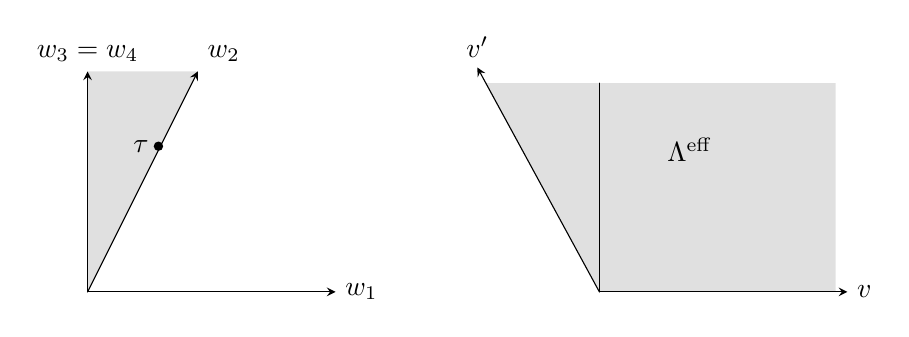
\begin{tikzpicture}[x=1.0cm,y=1.0cm,>=stealth,line cap=round,line join=round]
  \begin{scope}[shift={(-3.2,0)}]
    \fill[gray!24] (0,0) -- (0,2.8) -- (1.4,2.8) -- cycle;
    \draw[->] (0,0) -- (3.15,0) node[right] {$w_1$};
    \draw[->] (0,0) -- (0,2.8) node[above] {$w_3=w_4$};
    \draw[->] (0,0) -- (1.4,2.8) node[above right] {$w_2$};
    \fill (.9,1.85) circle (1.7pt) node[left] {$\tau$};
  \end{scope}
  \begin{scope}[shift={(3.3,0)}]
    \fill[gray!24] (0,0) -- (3.0,0) -- (3.0,2.65) -- (-1.45,2.65) -- cycle;
    \draw[->] (0,0) -- (3.15,0) node[right] {$v$};
    \draw[->] (0,0) -- (-1.55,2.85) node[above] {$v'$};
    \draw (0,0) -- (0,2.65);
    \node at (1.15,1.8) {$\Lambda^{\mathrm{eff}}$};
  \end{scope}
\end{tikzpicture}
\caption{作为商的环面簇。}\label{fig:11-3-1}
\end{figure}

在几何上，这个商流形是
\[
  M_\tau=
  \frac{\{x\in\mathbb C^4\mid
  |x_1|^2+|x_2|^2=2,\ |x_2|^2+|x_3|^2+|x_4|^2=3\}}
  {[x_1,x_2,x_3,x_4]\sim
  [e^{is}x_1,e^{i(s+t)}x_2,e^{it}x_3,e^{it}x_4]}.
\]
到 $S^2=\mathbb{CP}^1$ 的投影为
$[x_1,x_2,x_3,x_4]\mapsto[x_3:x_4]$。上同调类
$\overline w_\nu\in H^2(M_\tau)$ 是子流形
$\{x_\nu=0\}\subset M_\tau$ 的庞加莱对偶。因此，$\overline w_3=\overline w_4$ 是纤维类
$\phi\in H_2(M_\tau)$ 的庞加莱对偶，而 $\overline w_1,\overline w_2$ 是两个\BookRecordIndex{T0189}截面类
$\sigma_1,\sigma_2\in H_2(M_\tau)$ 的庞加莱对偶。这些类满足
\[
  \phi=\sigma_2-\sigma_1,
  \qquad \sigma_1\cdot\sigma_1=-1,
  \qquad \sigma_2\cdot\sigma_2=1,
  \qquad \phi\cdot\sigma_1=\phi\cdot\sigma_2=1.
\]
关系 $u_1u_2=q_1$ 表明：纤维类中通过两个截面和一个通有点的曲线之\BookRecordIndex{T0143}格罗莫夫--威滕
不变量为一。这可由直接观察明显看出。

这个流形的其他环面结构都不是 Fano 的；Spielberg \srcite{384} 证明，此时 Batyrev
公式不再成立。把这种\BookRecordIndex{T0229}量子上同调计算方法与 Ostrover \srcite{314} 的方法比较也颇有
启发。

\BookRecordIndex{T0169}环面流形的\BookRecordIndex{T0229}量子上同调环还可用 \BookRecordIndex{T0031}Landau--Ginzburg 势描述。（下面会在格拉斯曼流形的
情形解释这一表述。）即使在单调情形并采用适当域上的系数，这个环也未必半单；见
Ostrover--Tyomkin \srcite{316}。Fukaya--Oh--Ohta--Ono
\srcite{129, 130} 证明，它还与\BookRecordIndex{T0204}矩映射之环面纤维的拉格朗日\BookRecordIndex{T0132}弗洛尔同调密切相关。

\subsection{\BookRecordIndex{T0274}旗流形}\label{subsec:11-3-2}

Givental 和 Kim 在早期一篇优美论文 \srcite{153} 中计算了\BookRecordIndex{T0274}旗流形 $F_{n+1}$ 的\BookRecordIndex{T0229}量子上
同调环，并把它同 \BookRecordIndex{T0050}Toda 晶格联系起来。为此，他们对等变\BookRecordIndex{T0229}量子上同调的性质作了一些
假设，随后又在 \srcite{147, 210} 中证明了这些假设。Ciocan-Fontanine
\srcite{70} 给出了这个公式的另一种、更具代数意味的证明。这个例子引起了广泛兴趣，
既因为它与可积系统有非常直接的联系，也因为它和镜像对称有关。这些思想已推广到部分
\BookRecordIndex{T0274}旗流形；很好的参考资料是 Buch \srcite{49}。极端情形，即格拉斯曼流形 $G(k,n)$，将在
下一小节讨论。

\BookRecordIndex{T0274}旗流形 $F_{n+1}$ 是 $\mathbb C^{n+1}$ 中所有子空间列
\[
  E_1\subset E_2\subset\cdots\subset E_n,
  \qquad \dim_{\mathbb C}E_j=j,
\]
组成的空间。这个流形的实维数为 $n(n+1)$，它单连通，并带有自然复结构。把\BookRecordIndex{T0274}旗
$E_1\subset\cdots\subset E_n$ 映到 $E_1$ 的\BookRecordIndex{T0377}遗忘映射，是以 $F_n$ 为纤维、以
$\mathbb{CP}^n$ 为底的\BookRecordIndex{T0279}纤维化，由此可理解它的拓扑。例如，六维流形 $F_3$ 嵌入
$\mathbb{CP}^2\times\mathbb{CP}^2$，其像是满足关联关系 $\ell\subset P$ 的偶对
$(\ell,P)$ 所成的集合；这里把第二个 $\mathbb{CP}^2$ 看成
$\mathbb C^3$ 中复二维平面 $P$ 的空间。因此
\[
  F_3=\left\{([z_0:z_1:z_2],[w_0:w_1:w_2])\,\middle|\,
  \sum_i z_iw_i=0\right\}.
\]

\begin{remark}\label{rem:11-3-13}
虽然 $F_{n+1}$ 上有 $n$ 维环面的有效哈密顿作用，但即使在 $n=2$ 时它也不是\BookRecordIndex{T0169}环面流形，
因为 $2n<n(n+1)=\dim F_{n+1}$。另一方面，它可以实现为齐性空间
$U(n+1)/T^{n+1}$；也可表示为 $\mathbb C^N$ 关于群
$G:=U(1)\times\cdots\times U(n)$ 的哈密顿作用之辛商，其中
\[
  N:=\sum_{k=1}^n k(k+1).
\]
这是 Shaun Martin 向我们解释的。
\end{remark}

$F_{n+1}$ 的上同调由典范线丛
\[
  L_j:=E_{j+1}/E_j\longrightarrow F_{n+1},
  \qquad j=0,\ldots,n,
\]
的第一 Chern 类 $u_j\in H^2(F_{n+1};\mathbb Z)$ 生成。
\sourcefootnote{原书把这些类的所在空间误印为 $H^2(M;\mathbb Z)$；本段对象始终是
$F_{n+1}$，故补正。}
由于 Whitney 和 $L_0\oplus\cdots\oplus L_n$ 同构于平凡丛
$F_{n+1}\times\mathbb C^{n+1}$，这些类满足
\[
  u_0+\cdots+u_n=0.
\]
$F_{n+1}$ 的整个上同调环是商
\[
  H^*(F_{n+1})=
  \frac{\mathbb Z[u_0,\ldots,u_n]}
  {\langle\sigma_1(u),\ldots,\sigma_{n+1}(u)\rangle},
\]
其中 $\sigma_j(u)$ 是初等对称函数。为理解这一点，先注意上同调类
$c_j=\sigma_j(u)\in H^{2j}(F_{n+1})$ 是平凡丛
$L_0\oplus\cdots\oplus L_n$ 的 Chern 类，显然必须为零。上述公式断言，这些显然的关系
就是全部关系，而且 $F_{n+1}$ 的全部上同调都由 $u_j$ 通过杯积生成。一种证明方法是
考察\BookRecordIndex{T0279}纤维化序列
\[
  T\longrightarrow U\longrightarrow U/T\longrightarrow BT\longrightarrow BU,
\]
其中 $U:=U(n+1)$、$T:=T^{n+1}$，并把商 $U/T$ 与 $F_{n+1}$ 识别。诱导映射
$F_{n+1}:=U/T\to BT$ 把 $L_0\oplus\cdots\oplus L_n$ 分类为 $T$-丛。一个简单的谱序列
论证表明，$H^*(U/T)$ 中的关系由 $H^*(BU)$ 在 $H^*(BT)$ 中的像给出，也就是把 Chern
类写成变量 $u_i$ 的函数所得的关系。

$F_{n+1}$ 的上同调环还可用基
\[
  p_j=u_j+\cdots+u_n,
  \qquad j=1,\ldots,n
\]
表示。在这组基下，切丛 $TF_{n+1}$ 的第一 Chern 类为
\[
  c_1=2(p_1+\cdots+p_n).
\]
每个类 $p_j$ 都能由关于 $F_{n+1}$ 上显然复结构 $J$ \BookRecordIndex{T0058}半正的闭 $(1,1)$-形式代表。事实上，
上同调类 $a=\sum_j\lambda_jp_j$ 能由 凯勒 形式代表，当且仅当所有
$\lambda_j>0$。特别地，存在一个 凯勒 形式，使 $F_{n+1}$ 成为单调流形。还可\BookRecordIndex{T0326}推出：
对辛\BookRecordIndex{T0390}有效锥 $K^{\mathrm{eff}}(F_{n+1})\subset H_2(F_{n+1})$ 中的每个类 $A$，都有
$p_j(A)\geq0$；若 $A\ne0$，则至少有一个 $p_j(A)>0$。
\sourcefootnote{原书称每个 $p_j$ 本身由 凯勒 形式代表，并称
$\sum_j\lambda_jp_j$ 在 $\lambda_j\geq0$ 且其和为正时恰为 凯勒，进而断言每个
$p_j(A)>0$。但下一段的对偶基满足 $p_j(A_i)=\delta_{ij}$，在 $n>1$ 时直接排除这些
断言。$p_j$ 是到相应格拉斯曼流形之投影的 凯勒 类拉回，故本身仅\BookRecordIndex{T0058}半正；凯勒 锥的
内部条件是所有 $\lambda_j>0$，而有效类上的结论相应为逐项非负、非零类至少一项为正。}

令 $A_1,\ldots,A_n$ 是 $H_2(F_{n+1})$ 的整数基，它在
$p_j(A_i)=\delta_{ij}$ 的意义下与 $H^2(F_{n+1})$ 的基 $p_1,\ldots,p_n$ 对偶。我们使用
复系数，并取 $\Lambda:=\mathbb C[q_1,\ldots,q_n]$ 为\BookRecordIndex{T0231}量子系数环。定义~\ref{def:11-1-3}
中的同态 $\Gamma(F_{n+1})\to\Lambda(F_{n+1})$ 为
\[
  A\longmapsto e^A:=q^d:=q_1^{d_1}\cdots q_n^{d_n},
\]
其中 $d=(d_1,\ldots,d_n)$ 且 $d_j=p_j(A)\in\mathbb Z$。由于
$c_1=2(p_1+\cdots+p_n)$，每个 $q_i$ 的次数都是 $2c_1(A_i)=4$。简记
\[
  QH^*(F_{n+1}):=
  QH^*(F_{n+1};\mathbb C[q_1,\ldots,q_n])
  =H^*(F_{n+1})\otimes_{\mathbb Z}\mathbb C[q_1,\ldots,q_n].
\]
由于 $u_i$ 是 $H^*(F_{n+1})$ 的乘法生成元，一般原理（如下面
定理~\ref{thm:11-3-14} 的证明）表明，\BookRecordIndex{T0229}量子上同调环同构于多项式环
$\mathbb C[u_0,\ldots,u_n,q_1,\ldots,q_n]$ 的某个商。

Givental 和 Kim 在 \srcite{153} 中证明了自然同构
\[
  QH^*(F_{n+1})\cong
  \frac{\mathbb C[u_0,\ldots,u_n,q_1,\ldots,q_n]}{\mathcal I},
\]
其中理想 $\mathcal I$ 由下列矩阵的特征多项式各系数生成：
\[
  A_n=
  \begin{pmatrix}
    u_0&q_1&0&0&\cdots&0\\
    -1&u_1&q_2&0&\cdots&0\\
    0&-1&u_2&q_3&\ddots&\vdots\\
    \vdots&\ddots&\ddots&\ddots&\ddots&0\\
    0&\cdots&0&-1&u_{n-1}&q_n\\
    0&\cdots&\cdots&0&-1&u_n
  \end{pmatrix}.
\]
更明确地，考虑由公式
\[
  \det(A_n+\lambda\mathbf 1)
  =\lambda^{n+1}+c_1\lambda^n+\cdots+c_n\lambda+c_{n+1}
\]
确定的多项式 $c_j=\Sigma_j(u,q)$。理想 $\mathcal I$ 由这些函数 $\Sigma_j$ 生成。当
$q=0$ 时，它们就是初等对称函数
$\sigma_j(u)=\Sigma_j(u,0)$；因而在专门化到 $q=0$ 时，普通上同调环如预期般出现。换言
之，经典 Chern 类由初等对称函数给出，而多项式 $\Sigma_j$ 可视作 Chern 类的量子形变。

这个公式与可积哈密顿系统有一些很有意思的联系，现在加以说明。我们会看到，量子 Chern
类 $\Sigma_j$ 正是 \BookRecordIndex{T0050}Toda 晶格的 Poisson 对合积分；比较 \srcite{292}。

\BookRecordIndex{T0050}Toda 晶格是实直线上 $n+1$ 个单位质量质点的哈密顿微分方程，它们的位置为
$x_0,x_1,\ldots,x_n$。若
\[
  u_j=p_j-p_{j+1}=y_j=\dot x_j
\]
是位于 $x_j$ 的质点之动量，并且
\[
  q_j=e^{x_j-x_{j-1}},
\]
则 \BookRecordIndex{T0050}Toda 晶格的哈密顿函数为
\[
  H(x,y)=\frac12\operatorname{trace}(A_n^2)
  =\frac12\sum_{j=0}^ny_j^2-\sum_{j=1}^ne^{x_j-x_{j-1}}.
\]
（通常符号的反转对应于考察在 $x_0<x_1<\cdots<x_n$ 时相互排斥的力。）Moser 在
\srcite{292} 中发现，函数
$F_j(x,y)=\operatorname{trace}(A_n^j)$（$j=1,\ldots,n+1$）构成这个系统的一组完备
Poisson 对合积分。因此，由量子 Chern 类 $\Sigma_j$ 生成的理想 $\mathcal I$ 在 Poisson
括号下不变。

更精确地说，注意标准辛结构
$\omega=\sum_{j=0}^ndx_j\wedge dy_j$ 限制到零质心集合
$x_0+\cdots+x_n=0$ 和零动量集合 $y_0+\cdots+y_n=0$ 后，用变量
$q_1,\ldots,q_n,p_1,\ldots,p_n$ 写成
\[
  \omega=\frac{dq_1}{q_1}\wedge dp_1+\cdots+
  \frac{dq_n}{q_n}\wedge dp_n.
\]
Poisson 结构应相对于这个\BookRecordIndex{T0363}辛形式理解。

在几何上，\BookRecordIndex{T0363}辛形式 $\omega$ 可作如下解释。考虑复环面
\[
  T_{\mathbb C}:=H^2(F_{n+1};\mathbb C/2\pi i\mathbb Z)
  =\frac{H^2(F_{n+1};\mathbb C)}{H^2(F_{n+1};2\pi i\mathbb Z)},
\]
它由取值于 $\mathbb C^*=\mathbb C\setminus\{0\}$ 的坐标函数
\[
  q_j(a)=e^{\langle a,A_j\rangle}
\]
参数化。$T_{\mathbb C}$ 的余切丛可自然识别为
\[
  T^*T_{\mathbb C}
  =H^2(F_{n+1};\mathbb C/2\pi i\mathbb Z)
  \times H_2(F_{n+1};\mathbb C),
\]
其中 $p_j:H_2(F_{n+1};\mathbb C)\to\mathbb C$ 应理解为余切空间上的坐标函数。
\sourcefootnote{原书在这里把 $p_j$ 的定义域写成 $H_2(M;\mathbb C)$；本段所讨论的是
$T^*T_{\mathbb C}$，其余切纤维刚刚识别为 $H_2(F_{n+1};\mathbb C)$，故底空间应为
$F_{n+1}$。}
这些坐标函数
有上述 凯勒 形式锥所赋予的几何含义。形式 $\omega$ 可理解为余切丛
$T^*T_{\mathbb C}$ 上的复辛结构。在这种解释下，以上质点为
$x_0,\ldots,x_n$ 的哈密顿系统，在限制到零质心和零动量集合后，位于
$T^*T_{\mathbb C}$ 的实部上。

这给出\BookRecordIndex{T0229}量子上同调本身的一种几何解释。在识别
$u_j:=p_j-p_{j+1}$（$p_0=p_{n+1}=0$）下与 $\mathcal I$ 对应的理想
\[
  \mathcal J\subset\mathbb C[p_1,\ldots,p_n,q_1,\ldots,q_n]
\]
确定代数簇 $L\subset T^*T_{\mathbb C}$。这个簇定义为 $\mathcal J$ 中所有多项式的公共
零点集。因此，复系数\BookRecordIndex{T0229}量子上同调环
\[
  QH^*(F_{n+1})\cong
  \frac{\mathbb C[p_1,\ldots,p_n,q_1,\ldots,q_n]}{\mathcal J}
\]
可解释为 $L$ 上的函数空间。理想 $\mathcal J$ 在 Poisson 括号下的不变性，转化为簇
$L$ 是拉格朗日的这一条件。这初步展现了\BookRecordIndex{T0229}量子上同调中出现的结构（即镜像对称的所谓
“A 侧”）如何同“B 侧”相联；这也是 Givental 在 \srcite{148} 中证明\BookRecordIndex{T0274}旗流形镜像猜想时
所用的要素之一。

\subsection{格拉斯曼流形}\label{subsec:11-3-3}

格拉斯曼流形 $G(k,n)$ 的\BookRecordIndex{T0229}量子上同调环，已由 Bertram、Daskalopoulos 和 Wentworth
\srcite{36}、Witten \srcite{422} 以及 Siebert 和 Tian \srcite{378} 研究。Witten 在
\srcite{422} 中还把 $G(k,n)$ 的\BookRecordIndex{T0229}量子上同调同 $U(k)$ 表示的 Verlinde 代数联系起来。他
对这种联系的解释基于一个优美但启发式的路径积分考察。

以 $G(k,n)$ 表示 $\mathbb C^n$ 中 $k$ 维平面的格拉斯曼流形。因此，$G(k,n)$ 中一点是
$k$ 维子空间 $V\subset\mathbb C^n$。$V$ 的一个酉\BookRecordIndex{T0067}标架是矩阵
$B\in\mathbb C^{n\times k}$，满足
\[
  V=\operatorname{im}B,\qquad B^*B=\mathbf 1_{k\times k}.
\]
两个这样的\BookRecordIndex{T0067}标架 $B,B'$ 表示同一子空间 $V$，当且仅当存在酉矩阵 $U\in U(k)$ 使
$B'=BU$。所以格拉斯曼流形可与商空间
\[
  G(k,n)=\mathcal F(k,n)/U(k)
\]
识别，其中 $\mathcal F(k,n)\subset\mathbb C^{n\times k}$ 是所有酉 $k$-\BookRecordIndex{T0067}标架组成的集合。立即可见
\[
  \dim G(k,n)=2k(n-k).
\]

它也可解释为辛商或约化空间。空间 $\mathbb C^{n\times k}$ 是\BookRecordIndex{T0358}辛流形，群 $U(k)$ 在其上
的自然作用是哈密顿的，\BookRecordIndex{T0204}矩映射为 $\mu(B)=B^*B/2i$。要理解这一点，回忆\BookRecordIndex{T0204}矩映射取值于
$U(k)$ 李代数的对偶 $\mathfrak u(k)^*$；通过内积
$\langle\xi,\eta\rangle:=\operatorname{trace}(\xi^*\eta)$，可把它与
$\mathfrak u(k)$，即所有 $k\times k$ 斜埃尔米特矩阵的空间识别。于是
\[
  G(k,n)=\mu^{-1}(\mathbf 1/2i)/U(k).
\]

有两个自然复向量丛：秩 $k$ 的 $E\to G(k,n)$ 与秩 $n-k$ 的 $F\to G(k,n)$；它们的
Whitney 和自然同构于平凡丛 $G(k,n)\times\mathbb C^n$。在点 $V\in G(k,n)$ 处，$E$
的纤维就是 $V$ 本身，而 $F$ 的纤维是商 $\mathbb C^n/V$：
\[
  E_V=V,\qquad F_V=\mathbb C^n/V.
\]
把对偶丛 $E^*,F^*$ 的 Chern 类记为
\[
  x_j=c_j(E^*)\in H^{2j}(G(k,n)),
  \qquad
  y_j=c_j(F^*)\in H^{2j}(G(k,n)).
\]
这些类生成 $G(k,n)$ 的上同调。由于 $E\oplus F$ 同构于平凡丛，有显然的关系
\[
  \sum_{i=0}^j x_i y_{j-i}=0,
  \qquad j=1,\ldots,n,
\]
其中 $x_0=y_0=1$。当 $j>n$ 时，这个等式平凡地成立。对
$j=1,\ldots,n-k$，它通过
\[
  y_j=-x_1y_{j-1}-\cdots-x_{j-1}y_1-x_j,
  \qquad j=1,\ldots,n-k,
\]
把 $y_j$ 归纳地确定为 $x_1,\ldots,x_k$ 的函数。对 $j>n-k$，类 $y_j$ 为零，这给出
$x_j$ 之间的关系。这些就是全部关系，所以格拉斯曼流形的上同调环可与商
\[
  H^*(G(k,n);\mathbb C)\cong
  \frac{\mathbb C[x_1,\ldots,x_k]}
  {\langle y_{n-k+1},\ldots,y_n\rangle}
\]
识别。此外，切丛的第一 Chern 类为
$c_1(TG(k,n))=nx_1$，所以\BookRecordIndex{T0418}最小陈数为 $n$。

下述定理的本质内容由 Witten \srcite{422} 证明。Siebert 和 Tian
\srcite{378} 独立给出了包含全部细节的严格证明。

\begin{theorem}[Siebert--Tian、Witten]\label{thm:11-3-14}
以多项式环 $\mathbb C[q]$ 为系数的格拉斯曼流形\BookRecordIndex{T0229}量子上同调环同构于
\[
  QH^*(G(k,n);\mathbb C[q])
  \cong
  \frac{\mathbb C[x_1,\ldots,x_k,q]}
  {\langle y_{n-k+1},\ldots,y_{n-1},
  y_n+(-1)^{n-k}q\rangle}.
\]
这里 $x_j$ 是次数 $2j$ 的生成元，$q$ 是次数 $2n$ 的生成元。关系
$y_n+(-1)^{n-k}q=0$ 也可写成
\[
  x_ky_{n-k}=(-1)^{n-k}q.
\]
\end{theorem}

\begin{proof}
先指出，通过一个简单的归纳论证，$x_1,\ldots,x_k$ 仍生成 $G(k,n)$ 的\BookRecordIndex{T0229}量子上同调。这
意味着每个上同调类都能写成 $x_i$ 的量子积的线性组合。证明对次数归纳，并使用
$x*y-x\smile y$ 是次数严格低于 $x\smile y$ 的项之和这一事实。（细节见
\srcite{378, Lemma 2.1}。）同一论证还说明，经典上同调环中的原关系，通过加入若干低阶
项变成\BookRecordIndex{T0229}量子上同调中的关系。再次对次数归纳可知，这些新关系生成\BookRecordIndex{T0229}量子上同调中的关系理想。
（细节见 \srcite{378, Theorem 2.2}。）

据此，只需计算上同调环定义关系的量子形变。这里沿用 Witten 在 \srcite{422} 中的
论证。类 $x_i,y_j$ 的\BookRecordIndex{T0228}量子杯积是如下形式的幂级数：
\[
  x_i*y_j=\sum_d(x_i*y_j)_dq^d,
\]
其中
\[
  (x_i*y_j)_d\in H^{2i+2j-2nd}(G(k,n)),
  \qquad (x_i*y_j)_0=x_i\smile y_j.
\]
所以，除非 $i=k$ 且 $j=n-k$，\BookRecordIndex{T0228}量子杯积 $x_i*y_j$ 必须等于普通杯积
$x_i\smile y_j$。关系 $y_j=0$（$j=n-k+1,\ldots,n-1$）只涉及 $i<k$ 或
$j<n-k$ 的乘积 $x_iy_j$，因而在\BookRecordIndex{T0229}量子上同调中仍成立。不过，关系 $y_n=0$ 涉及乘积
$x_ky_{n-k}$，其量子形变唯一可能的非平凡贡献是
$(x_k*y_{n-k})_1\in H^0(G(k,n))$。我们断言
\begin{equation}\label{eq:11-3-19}
  (x_k*y_{n-k})_1=(-1)^{n-k}.
\end{equation}

为此，须考察次数
$\deg(u)=c_1(L)=1$ 的全纯曲线 $u:\mathbb{CP}^1\to G(k,n)$ 所成的\BookRecordIndex{T0246}模空间
$\mathcal M(L;J_0)$，其中 $J_0$ 是格拉斯曼流形的标准复结构。这个曲线空间的形式维数为
\[
  \dim\mathcal M(L;J_0)=2k(n-k)+2n.
\]
每条 $u\in\mathcal M(L;J_0)$ 都具有形式
\begin{equation}\label{eq:11-3-20}
  u([z_0:z_1])=\operatorname{span}
  \{z_0v_0+z_1v_1,v_2,\ldots,v_k\},
\end{equation}
其中 $v_0,\ldots,v_k\in\mathbb C^n$ 线性无关。这些映射确实组成一个维数为
$2n(k+1)-2k^2$ 的空间，与 $\mathcal M(L;J_0)$ 的维数公式一致。此外，由
命题~\ref{prop:7-4-3}，$J_0\in\mathcal J_{\mathrm{reg}}(G(k,n))$，所以
$\mathcal M(L;J_0)$ 中每条曲线都正则。

需要证明
\[
  \operatorname{GW}_{L,3}^M(x_k,y_{n-k},a)=(-1)^{n-k},
\]
其中 $a=\operatorname{PD}(\mathrm{pt})$ 生成 $H^{2k(n-k)}(G(k,n))$。
\sourcefootnote{原书把点类生成元所在空间写成 $M$；这里从\BookRecordIndex{T0246}模空间、曲线到插入类始终
讨论的是 $G(k,n)$，故应为 $H^{2k(n-k)}(G(k,n))$。}
向量丛的最高维 Chern
类之庞加莱对偶，可以用通有截面的零点集表示。例如，固定 $w\in\mathbb C^n$，考虑
截面 $G(k,n)\to E^*$，它给每个 $k$ 维平面 $V\subset\mathbb C^n$ 指派线性泛函
\[
  V\longrightarrow\mathbb C,\qquad v\longmapsto\langle w,v\rangle.
\]
这个截面横截于零截面，其零点集是子流形
\[
  X=\{V\in G(k,n)\mid w\perp V\}.
\]
这个子流形是 $G(k,n)$ 中的一份 $G(k,n-1)$，表示类
$\operatorname{PD}(x_k)\in H_{2k(n-k)-2k}(G(k,n))$。
\sourcefootnote{原书把这里的同调次数误印为 $2k$。零点集
$X\cong G(k,n-1)$ 的实维数为 $2k(n-k-1)=2k(n-k)-2k$，也正是次数 $2k$ 的类
$x_k$ 之庞加莱对偶的维数。}
再固定 $v_0\in\mathbb C^n$，考虑截面
$G(k,n)\to F$，它给每个 $V\in G(k,n)$ 指派等价类
$[v_0]\in\mathbb C^n/V=F_V$。其零点集是
\[
  Y=\{V\in G(k,n)\mid v_0\in V\}.
\]
这个子流形带自然定向，表示最高 Chern 类
$c_{n-k}(F)=(-1)^{n-k}c_{n-k}(F^*)$ 的庞加莱对偶。总之，
\[
  [X]=\operatorname{PD}(x_k),
  \qquad
  [Y]=(-1)^{n-k}\operatorname{PD}(y_{n-k}).
\]

任取 $V_0\in G(k,n)\setminus X$，使 $v_0\notin V_0$，并选取 $V_0$ 的一组基
$v_1,\ldots,v_k$，使 $v_2,\ldots,v_k$ 以及 $v_0+v_1$ 都垂直于 $w$。于是曲线
\[
  u([z_0:z_1])=\operatorname{span}
  \{z_0v_0+z_1v_1,v_2,\ldots,v_k\}
\]
满足
\[
  u([0:1])=V_0,\qquad u([1:1])\in X,\qquad u([1:0])\in Y.
\]
还容易看出，在 $u$ 处的相交数为一，并且没有另一条次数为一的曲线，其像同时与
$X,Y,V_0$ 相交。这算出同调不变量
$\operatorname{GW}_{L,3}^M(X,Y,\mathrm{pt})=1$，从而证明公式~\eqref{eq:11-3-19}。
所以在\BookRecordIndex{T0229}量子上同调中，形变后的关系为：当 $n-k+1\leq j\leq n-1$ 时 $y_j=0$，以及
$y_n+(-1)^{n-k}q=0$。定理~\ref{thm:11-3-14} 得证。
\end{proof}

定理~\ref{thm:11-3-14} 再次表明：若把 $q$ 看成复数而非变量，并专门化到 $q=0$，\BookRecordIndex{T0229}量子
上同调便退化为经典上同调环。更明确地，若定义 Chern 多项式
\[
  c_t(E^*)=1+\sum_{i=1}^kx_it^i,
  \qquad
  c_t(F^*)=1+\sum_{j=1}^{n-k}y_jt^j,
\]
\sourcefootnote{原书在这里及下文再次定义 $c_t(E^*)$ 时都从 $i=1$ 起求和，却同时使用
$c_t(E^*)c_t(F^*)=1$、$1/c_t(E^*)$ 以及式~\eqref{eq:11-3-22} 右端常数项为一的乘积。
因此两个 Chern 多项式都唯一缺少 $c_0=1$；这里及式~\eqref{eq:11-3-22} 补出常数项。}
则经典上同调环由关系 $c_t(E^*)c_t(F^*)=1$ 确定，而\BookRecordIndex{T0229}量子上同调环由
\begin{equation}\label{eq:11-3-21}
  c_t(E^*)c_t(F^*)=1+(-1)^{n-k}qt^n
\end{equation}
确定，其中 $q\in\mathbb C$。

\medskip
\noindent\textbf{Landau--Ginzburg 表述。}
经典上同调中的关系可以由单个函数
$W_0=W_0(x_1,\ldots,x_k)$ 的各偏导数生成。\BookRecordIndex{T0229}量子上同调中的关系也是如此，相应函数
$W=W(x_1,\ldots,x_k)$ 称为 \BookRecordIndex{T0031}Landau--Ginzburg 势。以下讨论紧随 Witten
\srcite{422} 的叙述。

考虑 Chern 多项式
\[
  c_t(E^*):=1+\sum_{i=1}^kx_it^i,
\]
其中 $x_i=c_i(E^*)\in H^{2i}(G(k,n))$。对 $j\geq0$，以公式
\[
  \frac1{c_t(E^*)}:=\sum_{j\geq0}y_jt^j
\]
定义多项式 $y_j=y_j(x_1,\ldots,x_k)$。于是格拉斯曼流形的经典上同调环由关系
$y_j(x)=0$（$n-k+1\leq j\leq n$）描述。这些关系蕴含当 $j>n$ 时
$y_j(x)=0$；当然，当 $1\leq j\leq n-k$ 时，$y_j$ 正是 $F^*$ 的 Chern 类。以下不施加
关系 $y_j(x)=0$，所以幂级数 $\sum_jy_jt^j$ 未必还是多项式。

考虑由等式
\[
  -\log c_t(E^*):=\sum_{r\geq0}U_r(x)t^r
\]
定义的全纯函数 $U_r=U_r(x_1,\ldots,x_k)$。对这个表达式关于 $x_j$ 求导，得到
\[
  -\frac{t^j}{c_t(E^*)}
  =\sum_{r\geq0}\frac{\partial U_r}{\partial x_j}t^r.
\]
比较系数可知，对 $1\leq j\leq k$，
$\partial U_r/\partial x_j=-y_{r-j}$。特别地，当 $r-j<0$ 时，该公式说明 $U_r$ 的相应
偏导数为零。最有意义的是 $r=n+1$。令
\[
  W_0:=(-1)^{n+1}U_{n+1},
\]
便有
\[
  \frac{\partial W_0}{\partial x_j}=(-1)^ny_{n+1-j},
  \qquad 1\leq j\leq k.
\]
所以格拉斯曼流形经典上同调的定义关系可以写成 $dW_0=0$。

现在考虑函数
\[
  W:=W_0+(-1)^kqx_1,
\]
其中 $q$ 是固定复数。条件 $dW=0$ 等价于
\[
  y_{n-k+1}=0,\quad\ldots,\quad y_{n-1}=0,
  \quad y_n+(-1)^{n-k}q=0,
\]
恰好就是 $G(k,n)$ \BookRecordIndex{T0229}量子上同调环的定义关系。注意，幂级数
$\sum_jy_jt^j$ 的高阶系数不再消失。比较等式
$c_t(E^*)\bigl(\sum_{j\geq0}y_jt^j\bigr)=1$ 中不超过 $n$ 阶的系数，得到
\[
  \left(1+\sum_{i=1}^kx_it^i\right)
  \left(1+\sum_{j=1}^{n-k}y_jt^j\right)
  =1+(-1)^{n-k}qt^n,
\]
这与式~\eqref{eq:11-3-21} 一致。

函数 $W$ 称为 \BookRecordIndex{T0031}Landau--Ginzburg 势。用 Chern 多项式的根
$\lambda_1,\ldots,\lambda_k$ 可方便地表示它：
\begin{equation}\label{eq:11-3-22}
  c_t(E^*)=1+\sum_{i=1}^kx_it^i
  =\prod_{i=1}^k(1+\lambda_it),
\end{equation}
即
\begin{equation}\label{eq:11-3-23}
  W(\lambda_1,\ldots,\lambda_k)
  =\sum_{i=1}^k\left(\frac{\lambda_i^{n+1}}{n+1}
  +(-1)^kq\lambda_i\right).
\end{equation}
从几何上说，$G(k,n)$ 的\BookRecordIndex{T0229}量子上同调环可解释为变量 $x_1,\ldots,x_k$ 的多项式限制到
$dW$ 零点集后所得的环。函数 $W:\mathbb C^k\to\mathbb C$ 只有有限多个\BookRecordIndex{T0233}临界点，而且任意
多项式 $f\in\mathbb C[x_1,\ldots,x_k]$ 模理想
\[
  \mathcal J_q:=
  \langle y_{n-k+1},\ldots,y_{n-1},y_n+(-1)^{n-k}q\rangle
  =\left\langle\frac{\partial W}{\partial x_1},\ldots,
  \frac{\partial W}{\partial x_k}\right\rangle
\]
的等价类，由 $f$ 在 $W$ 的\BookRecordIndex{T0233}临界点处的值确定。由此得到如下局部化公式：
\begin{equation}\label{eq:11-3-24}
  I(f)=\frac{(-1)^{k(k-1)/2}}{k!}
  \sum_{dW(x)=0}
  \det\left(\frac{\partial^2W}{\partial x_i\partial x_j}\right)^{-1}f(x),
\end{equation}
它对每个次数为 $2k(n-k)$ 的多项式 $f$ 成立。这里把变量 $x_i$ 理解为次数 $2i$，而
泛函 $I(f)$ 表示微分形式
$\omega_f\in\Omega^{2k(n-k)}(G(k,n))$ 的积分；该形式在同构
\[
  H^*(G(k,n);\mathbb C)
  =\frac{\mathbb C[x_1,\ldots,x_k]}{\langle dW_0\rangle}
\]
下与 $f$ 对应。注意，$f$ 所表示的\BookRecordIndex{T0229}量子上同调类
$c_f\in QH^*(G(k,n))$ 是 $[\omega_f]$ 与含 $q$ 的项之和。

\begin{exercise}\label{ex:11-3-15}
通过考察 $G(k,n)$ 中 $n-k$ 份 $G(k,n-1)$ 的交点，证明
\[
  \int_{G(k,n)}c_k(E^*)^{n-k}=1.
\]
再把公式~\eqref{eq:11-3-24} 用于多项式
\[
  f(x)=x_k^{n-k}=\prod_{i=1}^k\lambda_i^{n-k},
\]
验证该公式；这个多项式表示类 $c_k(E^*)^{n-k}$。由于
$H^{2k(n-k)}(G(k,n))$ 是一维的，一般情形由此即得。

提示：先作变量替换，并用留数演算把和式~\eqref{eq:11-3-24} 写成如下围道积分：
\[
  I(f)=\frac{(-1)^{k(k-1)/2}}{k!(2\pi i)^k}
  \int_{|\lambda_j|=R}
  \frac{f\prod_{i<j}(\lambda_i-\lambda_j)^2}
  {\prod_i\partial W/\partial\lambda_i}
  \,d\lambda_1\cdots d\lambda_k,
\]
其中 $R$ 很大。然后注意，分母中的
$\partial W/\partial\lambda_i=\lambda_i^n+(-1)^kq$ 可由
$\lambda_i^n-\lambda_i^{n-k}$ 代替而不改变积分值。再用一次留数演算求出新积分。细节见
\srcite{422} 和 \srcite{378}。
\end{exercise}

\medskip
\noindent\textbf{同 Verlinde 代数的关系。}
格拉斯曼流形 $G(k,n)$ 的上同调环与酉群 $U(k)$ 表示环的一个适当商之间，有一种非凡的
对应，下面加以说明。作为实向量空间，$G(k,n)$ 的上同调由 Schubert 循环生成。
$G(k,n)$ 中的一个 Schubert 循环，是与一面完全\BookRecordIndex{T0274}旗
\[
  \{0\}=\Lambda_0\subset\Lambda_1\subset\cdots\subset
  \Lambda_{n-1}\subset\Lambda_n=\mathbb C^n,
  \qquad \dim_{\mathbb C}\Lambda_\nu=\nu,
\]
以及一个非负整数的有限序列（称为分拆）
\[
  n-k\geq a_1\geq a_2\geq\cdots\geq a_k\geq0
\]
相联系的子流形。相应子流形
\[
  \Sigma_a:=\Sigma_a(\Lambda)=
  \Sigma_{a_1,\ldots,a_k}^{k,n}(\Lambda_0,\ldots,\Lambda_n)
  \subset G(k,n)
\]
由所有满足
\[
  \dim(V\cap\Lambda_{n-k+i-a_i})=i,
  \qquad
  \dim(V\cap\Lambda_{n-k+i-a_i-1})=i-1,
\]
$i=1,\ldots,k$ 的 $k$ 维子空间 $V\subset\mathbb C^n$ 组成。换言之，维数列
$\dim(V\cap\Lambda_\nu)$ 在 $\nu=n-k+i-a_i$ 处增加一。每个 Schubert 循环
$\Sigma_a(\Lambda)$ 都是 $G(k,n)$ 中复余维
\[
  \operatorname{codim}_{\mathbb C}\Sigma_a
  =a_1+\cdots+a_k=:|a|
\]
的光滑子流形。它的闭包为
\[
  \overline\Sigma_a=\bigcup_{b\succeq a}\Sigma_b,
  \qquad b\succeq a\quad\Longleftrightarrow\quad b_i\geq a_i
  \text{ 对所有 }i.
\]
\sourcefootnote{原书把闭包关系误印为 $b\preceq a$ 且 $b_i\leq a_i$。但由上面的精确跃迁
条件，闭包只能加入更特殊、余维更高的 Schubert 胞\BookRecordIndex{T0280}腔，即 $b_i\geq a_i$；例如
$G(1,2)$ 中 $a=1$ 的胞\BookRecordIndex{T0280}腔本身已是闭点。}
因此，$\Sigma_a$ 是定义~\ref{def:6-5-1} 意义下的\BookRecordIndex{T0337}伪循环，从而通过相交数表示同调类
\[
  \sigma_a:=[\Sigma_a]
  \in H_{2k(n-k)-2|a|}(G(k,n));
\]
见引理~\ref{lem:6-5-7}。这些同调类加法生成 $H_*(G(k,n))$，所以
\[
  \dim H_*(G(k,n))=\binom nk.
\]
此外，对两面通有\BookRecordIndex{T0274}旗 $\Lambda,\Lambda'$，Schubert 循环
$\Sigma_a(\Lambda)$ 与 $\Sigma_b(\Lambda')$ 横截相交；若二者维数互补，则
\[
  g_{ab}:=\sigma_a\cdot\sigma_b=
  \begin{cases}
    1,&a_{k+1-i}+b_i=n-k\text{ 对所有 }i,\\
    0,&\text{否则}.
  \end{cases}
\]
这些断言的证明见 Griffiths--Harris \srcite{159} 与 Milnor--Stasheff
\srcite{291}。

\begin{remark}\label{rem:11-3-16}
用 Schubert 循环表示，上同调类 $x_i,y_j$ 为
\[
  x_i=c_i(E^*)=\operatorname{PD}(\xi_i),
  \qquad
  y_j=c_j(F^*)=(-1)^j\operatorname{PD}(\eta_j),
\]
其中
\[
  \xi_i:=\sigma_{\underbrace{1,\ldots,1}_{i\text{ 次}},0,\ldots,0},
  \qquad
  \eta_j:=\sigma_{j,0,\ldots,0}.
\]
\end{remark}

\begin{remark}[Giambelli 公式]\label{rem:11-3-17}
固定整数 $n-k\geq a_1\geq\cdots\geq a_k\geq0$，并以
\[
  b_j:=\#\{i\mid a_i\geq j\}
\]
定义整数 $k\geq b_1\geq\cdots\geq b_{n-k}\geq0$。则
\[
  \sigma_a=
  \det\begin{pmatrix}
    \eta_{a_1}&\eta_{a_1+1}&\cdots&\eta_{a_1+k-1}\\
    \eta_{a_2-1}&\eta_{a_2}&\cdots&\eta_{a_2+k-2}\\
    \vdots&\vdots&\ddots&\vdots\\
    \eta_{a_k-k+1}&\eta_{a_k-k+2}&\cdots&\eta_{a_k}
  \end{pmatrix}.
\]
同一个类也可写成
\[
  \sigma_a=
  \det\begin{pmatrix}
    \xi_{b_1}&\xi_{b_1+1}&\cdots&\xi_{b_1+n-k-1}\\
    \xi_{b_2-1}&\xi_{b_2}&\cdots&\xi_{b_2+n-k-2}\\
    \vdots&\vdots&\ddots&\vdots\\
    \xi_{b_{n-k}-n+k+1}&\xi_{b_{n-k}-n+k+2}&\cdots&\xi_{b_{n-k}}
  \end{pmatrix}.
\]
这里的乘法应理解为相交积。
\end{remark}

群 $U(k)$ 的表示环 $\mathcal R(k)$ 定义为表示偶对 $\rho\mathbin\#\rho'$ 如 K 理论般取
等价类所得的集合。表示 $\rho:U(k)\to\operatorname{Aut}(V)$ 的特征标，是最大环面
$T^k\subset U(k)$ 上的函数
\[
  \theta_\rho:T^k\longrightarrow\mathbb C,
  \qquad \theta_\rho(t):=\operatorname{trace}_{\mathbb C}(\rho(t)).
\]
由于具有相同对角元、只差排列的两个对角矩阵彼此共轭，特征标是 $t$ 的坐标
$t_1,\ldots,t_k$ 的对称函数。特征标给出环同构
\[
  \mathcal R(k)\longrightarrow\mathcal S(k),
  \qquad \rho\longmapsto\theta_\rho,
\]
这里表示环采用直和与张量积，而 $\mathcal S(k)$ 是 $k$ 个变量的对称函数环。每个分拆
$a_1\geq\cdots\geq a_k\geq0$ 都确定一个不可约表示
$\rho_a:U(k)\to\operatorname{Aut}(V_a)$，在同构意义下唯一；它的特征标是下面
注~\ref{rem:11-3-19} 所定义的函数 $\theta_{\rho_a}=\theta_a$。明确地，表示空间 $V_a$
是子空间
\[
  V_a\subset
  (\Lambda^1\mathbb C^k)^{\otimes m_1}\otimes
  (\Lambda^2\mathbb C^k)^{\otimes m_2}\otimes\cdots\otimes
  (\Lambda^k\mathbb C^k)^{\otimes m_k},
\]
其中 $m_i:=a_i-a_{i+1}$；它定义为包含 $T^k$-不变子空间之张量积
\[
  (\mathbb Ce_1\wedge\cdots\wedge\mathbb Ce_i)^{\otimes m_i}
\]
的最小 $U(k)$-不变子空间。

\begin{remark}\label{rem:11-3-18}
特别有意义的是特殊表示
\[
  V_{\underbrace{1,\ldots,1}_{i\text{ 次}},0,\ldots,0}
  =\Lambda^i\mathbb C^k,
  \qquad
  V_{j,0,\ldots,0}=S^j\mathbb C^k.
\]
特别地，$V_{0,\ldots,0}=\mathbb C$ 是平凡表示，即表示环的乘法单位元。
\end{remark}

\begin{remark}[Jacobi--Trudi 恒等式]\label{rem:11-3-19}
在变量 $t_1,\ldots,t_k$ 中，对 $1\leq i\leq k$ 定义初等对称函数 $\phi_i$，对
$j\geq1$ 定义完全对称函数 $\psi_j$：
\[
  \phi_i=\sum_{1\leq\nu_1<\cdots<\nu_i\leq k}
  t_{\nu_1}\cdots t_{\nu_i},
  \qquad
  \psi_j=\sum_{1\leq\nu_1\leq\cdots\leq\nu_j\leq k}
  t_{\nu_1}\cdots t_{\nu_j}.
\]
令 $a_i,b_j$ 如注~\ref{rem:11-3-17}，并定义对称函数
\[
  \theta_a:=
  \frac{\det(t_i^{a_j+k-j})_{i,j=1}^k}
  {\det(t_i^{k-j})_{i,j=1}^k}.
\]
则
\[
  \theta_a=
  \det\begin{pmatrix}
    \psi_{a_1}&\psi_{a_1+1}&\cdots&\psi_{a_1+k-1}\\
    \psi_{a_2-1}&\psi_{a_2}&\cdots&\psi_{a_2+k-2}\\
    \vdots&\vdots&\ddots&\vdots\\
    \psi_{a_k-k+1}&\psi_{a_k-k+2}&\cdots&\psi_{a_k}
  \end{pmatrix}.
\]
等价地，
\[
  \theta_a=
  \det\begin{pmatrix}
    \phi_{b_1}&\phi_{b_1+1}&\cdots&\phi_{b_1+n-k-1}\\
    \phi_{b_2-1}&\phi_{b_2}&\cdots&\phi_{b_2+n-k-2}\\
    \vdots&\vdots&\ddots&\vdots\\
    \phi_{b_{n-k}-n+k+1}&\phi_{b_{n-k}-n+k+2}&\cdots&\phi_{b_{n-k}}
  \end{pmatrix}.
\]
\end{remark}

环 $\mathcal R(k)$ 由不可约表示 $\rho_a$ 加法生成。考虑 $\mathcal R(k)$ 的有限维商
$\mathcal R(k,n)$，它由满足
$n-k\geq a_1\geq\cdots\geq a_k\geq0$ 的不可约表示 $\rho_a$ 生成。由
注~\ref{rem:11-3-17} 和注~\ref{rem:11-3-19}，有环同构
\begin{equation}\label{eq:11-3-25}
  H^*(G(k,n))\longrightarrow\mathcal R(k,n),
  \qquad \operatorname{PD}(\sigma_a)\longmapsto\rho_a.
\end{equation}
逆同构可描述如下。特征标
$\theta_\rho:=\operatorname{trace}_{\mathbb C}\circ\rho:U(k)\to\mathbb C$ 是特征值的
对称多项式，因而\BookRecordIndex{T0333}唯一延拓为 $\mathbb C^{k\times k}$ 上共轭不变的多项式。再把这个延拓
限制到李代数 $\mathfrak u(k)$。固定\BookRecordIndex{T0103}典范丛 $E\to G(k,n)$ 上的一个 $U(k)$-联络 $A$，
并以
\[
  F_A\in\Omega^2(G(k,n);\operatorname{End}(E))
\]
表示其曲率。于是 $\theta_\rho(F_A/2\pi i)$ 是 $G(k,n)$ 上闭的实值
$2|a|$-形式，表示丛 $E$ 的一个示性类。事实证明，
\[
  [\theta_a(F_A/2\pi i)]=\operatorname{PD}(\sigma_a),
\]
\sourcefootnote{原书在这个等式中把联络 $A$ 的曲率 $F_A$ 误印为 $F_a$；前一句定义以及
紧接着的逆同构都唯一确定下标应为大写 $A$。}
所以逆同构由映射
\[
  \mathcal R(k)\longrightarrow H^*(G(k,n)),
  \qquad \rho\longmapsto[\theta_\rho(F_A/2\pi i)]
\]
诱导。这些观察见 Witten 的论文 \srcite{422}。（亦见 Salamon \srcite{354} 的介绍。）
注意，这个同构把 $x_i$ 映到 $\Lambda^i\mathbb C^k$，把 $y_j$ 映到
$S^j\mathbb C^k$；见注~\ref{rem:11-3-16} 与注~\ref{rem:11-3-18}。

Verlinde 代数是 $\mathcal R(k,n)$ 上环结构的形变，正如\BookRecordIndex{T0229}量子上同调是
$H^*(G(k,n))$ 上杯积的形变。Verlinde 代数的结构常数，定义为平坦 $U(k)$-联络\BookRecordIndex{T0246}模空间
上某些向量丛的全纯 Euler 示性数；这些\BookRecordIndex{T0246}模空间与一个整数 $d$ 及三个表示
$\rho_a,\rho_b,\rho_c$ 相联系，而三者满足同三点\BookRecordIndex{T0143}格罗莫夫--威滕不变量一样的维数条件：
\[
  |a|+|b|+|c|=k(n-k)+nd.
\]
Witten 的猜想断言，同构~\eqref{eq:11-3-25} 交织这两种形变后的乘积结构。该猜想还推广
到高亏格\BookRecordIndex{T0143}格罗莫夫--威滕不变量及相应的高亏格 Verlinde 代数。其动机之一是，Verlinde
\BookRecordIndex{T0254}粘合规则与\BookRecordIndex{T0143}格罗莫夫--威滕不变量的\BookRecordIndex{T0254}粘合规则相同。此外，Witten 用路径积分给出了一个
优美的启发式论证，解释为何应有这种对应 \srcite{422}。对\BookRecordIndex{T0229}量子上同调，Agnihotri
\srcite{9} 已证实这个猜想；与定理~\ref{thm:11-3-14} 的证明一样，论证归结为计算单个
不变量。

\begin{remark}[结构常数]\label{rem:11-3-20}
定理~\ref{thm:11-3-14} 那样的同构，并不给出\BookRecordIndex{T0229}量子上同调结构常数
\[
  N_d(a,b,c):=\operatorname{GW}_{dL,3}^M(a,b,c)
\]
的显式公式。这一点在普通上同调中已经显现。例如，虽然
$H^*(G(k,n))$ 很容易写成多项式环的商，其结构常数
\[
  N_0(a,b,c)=\sigma_a\cdot\sigma_b\cdot\sigma_c
  =\frac1{\operatorname{Vol}(G)}
  \int_G\theta_a(g)\theta_b(g)\theta_c(g)\det(g)^{k-n}\,dg
\]
（积分相对于 $G=U(k)$ 上的 Haar 测度理解），却由 Littlewood--Richardson 规则确定；
这些规则涉及 Young 表上的相当复杂的操作。这样的公式还没有推广到一般的 $d$。
\end{remark}

\subsection{Calabi--Yau 流形}\label{subsec:11-3-4}

一般\BookRecordIndex{T0058}半正\BookRecordIndex{T0358}辛流形的\BookRecordIndex{T0229}量子上同调环 $QH^*(M)$ 中，会出现一些单调情形没有的有趣现象。例如，
定义~\ref{def:11-1-3} 中的\BookRecordIndex{T0231}量子系数环 $\Lambda$ 一般不能再取成多项式环，而须像
例~\ref{ex:11-1-4}（iv）、（v）那样使用 Novikov 环 $\Lambda_\omega$ 或\BookRecordIndex{T0270}普适 Novikov
环。一个重要特例是第一 Chern 类为零的\BookRecordIndex{T0358}辛流形。此时
$\Lambda=\Lambda_0$，即 $\Lambda$ 中所有元素的次数都为零，并且
\[
  QH^k(M;\Lambda)=H^k(M)\otimes\Lambda.
\]

进一步限制到六维情形。此时\BookRecordIndex{T0246}模空间 $\mathcal M(A;J)/G$ 的维数
$\dim M+2c_1(A)-6$ 对每个类 $A$ 都为零，所以对通有\BookRecordIndex{T0088}殆复结构 $J$，每条单纯
\BookRecordIndex{T0003}$J$-全纯曲线都是孤立的。由此，三点不变量
$\operatorname{GW}_{A,3}^M(a_1,a_2,a_3)$ 只有在所有 $\deg(a_i)=2$ 时才可能非零。事实上，
条件~\eqref{eq:7-1-2} 表明这些次数之和必须为六；另一方面还必须有 $\deg(a_i)\leq2$，因为否则
庞加莱对偶 $\operatorname{PD}(a_i)$ 可由维数小于四的循环表示，而由于非常值
\BookRecordIndex{T0003}$J$-全纯曲线都是孤立的，可把这个循环选成避开所有这些曲线。因此，除 $H^2(M)$ 上之外，
量子积都等于通常的乘积。此外，它诱导乘法
\[
  H^2(M)\otimes H^2(M)\longrightarrow H^4(M)\otimes\Lambda.
\]
用庞加莱对偶把 $H^2(M)$ 与 $H^4(M)$ 识别，便在
$QH^2(M;\Lambda)=H^2(M)\otimes\Lambda$ 上得到一个形变乘积结构。

满足上述条件的流形包括六维环面 $T^6$，以及乘积 $T^2\times X$，其中
$X\subset\mathbb{CP}^3$ 是四次超曲面（著名的 K3 曲面）。在这两种情形，\BookRecordIndex{T0143}格罗莫夫--
威滕不变量都消失。不过，还有一大类量子积非平凡、而且单连通并且是 凯勒 的例子。
这些流形称为 Calabi--Yau 三维簇。Yau 的一个定理表明，它们容许 Ricci 张量为零的
凯勒 度量，即所谓 Kähler--Einstein 度量。Calabi--Yau 三维簇是现代场论的基本材料，
因而受到物理学家和数学家的广泛研究；例如见 Candelas--Ossa \srcite{57}、
Bryan--Pandharipande \srcite{48}，以及 Cox--Katz \srcite{76} 中的参考文献。

它们的性质相当复杂。例如，人们或许希望，任意 Calabi--Yau 三维簇上的复结构 $J$ 都可
在可积复结构类中形变为复结构 $J'$，使每个给定同调类中只有有限多条
$J'$-全纯曲线。（$M$ 上的通有\BookRecordIndex{T0088}殆复结构确实有这个性质。）然而事实并非如此：P.~M.~H.
Wilson 在 \srcite{419} 中给出了一个显式反例。

Calabi--Yau 三维簇可作为环面四维簇中的超曲面出现，也可作为射影空间中的完全交出现。
下面更详细地研究 $\mathbb{CP}^4$ 中超曲面的特殊情形。由这种方式定义的流形 $(M,J)$
自然成族出现：当定义方程变化时，复结构也随之变化。镜像对称猜想的各种表述都体现如下
直觉：由某个特定 Calabi--Yau 流形 $(M,\omega)$ 的辛结构产生的结构（例如\BookRecordIndex{T0143}格罗莫夫--
威滕不变量，即 A 侧），应当在 $M$ 上复结构 $J$ 的形变所产生的结构（即 B 侧）中有其
对应物。这个猜想的推论之一，是 Candelas--Ossa--Green--Parkes \srcite{58} 对
$\mathbb{CP}^4$ 中五次超曲面上\BookRecordIndex{T0091}单纯曲线数作出的惊人预言。这个猜想的精确性引起了极大
兴趣；同样令人瞩目的是，它建立在当时对数学来说全新的思想之上。把这些思想置于坚实
基础上的努力，是推动本章所述诸多发展的力量之一。

更确切地，回忆上文，量子积在 $H^2(M)\otimes\Lambda$ 上诱导一个乘法。在 凯勒
情形，还可限制到 $H^{1,1}(M)\otimes\Lambda$，因为乘积在 $H^{2,0}$ 和 $H^{0,2}$ 上
平凡。另一方面，$M$ 上复结构的形变环是在 $H^{1,2}$ 上的环结构，它给出一个类似于
下文 WDVV 方程的微分方程。镜像对称猜想的一种表述断言：与每个 Calabi--Yau 流形 $M$
相伴，都有一个镜像流形 $M^*$，使环 $H^{1,1}(M^*)$ 与 $H^{1,2}(M)$ 自然同构。
Givental \srcite{150} 对 $\mathbb{CP}^4$ 中的五次超曲面，以及更一般的\BookRecordIndex{T0169}环面流形中完全
交，证实了这个猜想。事实上 Givental 证明了远不止这些，因为对应还保持两侧丰富得多的
结构。第~\ref{sec:11-5} 节会描述 A 侧的部分附加结构，而完整信息还包括
注~\ref{rem:7-5-4} 所提到的\BookRecordIndex{T0378}引力后裔。更多镜像对称资料见 Cox--Katz \srcite{76} 与
Voisin \srcite{409}。

\medskip
\noindent\textbf{$\mathbb{CP}^4$ 中的五次超曲面。}
考虑 $\mathbb{CP}^4$ 中的 $k$ 次超曲面
\[
  Z_k:=\left\{[z_0:\cdots:z_4]\in\mathbb{CP}^4\,\middle|\,
  \sum_{j=0}^4z_j^k=0\right\}.
\]
这个流形单连通，其 Betti 数为
\[
  b_2=b_4=1,
  \qquad
  b_3=k^4-5k^3+10k^2-10k+4.
\]
特别地，等式 $b_2=b_4=1$ 来自超平面截面的 Lefschetz 定理。因此
\[
  \pi_2(Z_k)\cong H_2(Z_k)\cong\mathbb Z,
\]
所以\BookRecordIndex{T0363}辛形式 $\omega$ 在 $\pi_2(Z_k)$ 上不为零。
\sourcefootnote{原书在这句话中先把 $H_2(Z_k)$ 误印为 $H_2(M)$，随后又把
$\pi_2(Z_k)$ 漏写下标为 $\pi_2(Z)$；本段固定对象均为超曲面 $Z_k$，故统一补正。}
此外，$Z_k$ 的第一 Chern 类为
\[
  c_1=(5-k)\iota^*h,
\]
其中 $h\in H^2(\mathbb{CP}^4;\mathbb Z)$ 是 $\mathbb{CP}^4$ 上同调的标准生成元，而
$\iota:Z_k\to\mathbb{CP}^4$ 是把 $Z_k$ 作为超曲面嵌入的自然映射。

令 $A\in\pi_2(Z_k)$ 是满足 $\omega(A)>0$ 的同伦群生成元。例如，当 $k$ 为奇数时，
$A$ 有显式全纯代表
\[
  [z_0:z_1]\longmapsto[z_0:z_1:-z_0:-z_1:0].
\]
在所有情形，$A$ 都由 $Z_k$ 中的一条直线表示。因此在这个生成元上计算第一 Chern 类
得到
\[
  c_1(A)=5-k.
\]
所以当 $k\leq4$ 时，流形 $Z_k$ 单调。当 $k>5$ 时，对通有\BookRecordIndex{T0088}殆复结构不存在非常值
\BookRecordIndex{T0003}$J$-全纯曲线，因为 $\omega$ 为正的类都有负 Chern 数；由维数原因，它们对通有 $J$
没有代表。

因此最有意义的是第一 Chern 类为零的五次超曲面 $M=Z_5$。这是 Calabi--Yau 流形的
典型例子。为了计算量子积，需要算出所有非零不变量
$\operatorname{GW}_{dA,3}^M(a_1,a_2,a_3)$。由于 $b_2=1$，只需计算
$\operatorname{GW}_{dA,3}^M(h,h,h)$；这里 $h$ 是超平面\BookRecordIndex{T0189}截面类
\[
  H=[Z_5\cap\mathbb{CP}^3]\in H_4(Z_5)
\]
的庞加莱对偶。因此 $h$ 就是前面记为 $\iota^*h$ 的类，并满足 $h(A)=1$。注意，对通有
（殆复）$J$，\BookRecordIndex{T0091}单纯曲线都是孤立的。因此，对每个 $\ell$，类 $\ell A$ 中单纯
\BookRecordIndex{T0003}$J$-全纯曲线的数目 $N_\ell$ 有限。既然这些曲线是基本几何对象，我们希望用数 $N_\ell$
表示 $\operatorname{GW}_{dA,3}^M(h,h,h)$。

回忆注~\ref{rem:7-3-8}，按定义
\[
  \operatorname{GW}_{dA,3}^M(h,h,h)
  =d^3\operatorname{GW}_{dA,0}^M,
\]
其中 $\operatorname{GW}_{dA,0}^M$ 是格罗莫夫--威滕过程所计数的 $dA$ 类曲线数。这个
不变量并不直接计数 \BookRecordIndex{T0003}$J$-全纯曲线，而是计数某个\BookRecordIndex{T0209}柯西--黎曼方程的图；在该方程中 $J$
依赖于 $z$。我们的目标是理解单纯 \BookRecordIndex{T0003}$J$-全纯曲线的多重覆盖如何贡献于
$\operatorname{GW}_{dA,0}^M$。

先注意，因为 $Z_5$ 是 $\mathbb{CP}^4$ 中次数为五的超曲面，
\[
  \operatorname{GW}_{0,3}^M(h,h,h)
  =H\cdot H\cdot H=[\mathbb{CP}^1]\cdot Z_5=5.
\]
此外，若 $C$ 是 $dA$ 类中的\BookRecordIndex{T0091}单纯曲线，则 $C\cdot H=d$。所以，把 $H$ 扰动到一般位置
后，$C$ 与 $H$ 横截地交于 $d$ 个不同点。因此，曲线 $C$ 对
$\operatorname{GW}_{dA,3}^M(h,h,h)$ 的贡献恰为 $d^3$。

现在考察 $C$ 的 $m$ 重覆盖对 $\operatorname{GW}_{mdA,3}^M(h,h,h)$ 的贡献。
\sourcefootnote{原书在此把不变量的曲线类印为 $dA$；但 $C$ 本身属于 $dA$，其 $m$ 重覆盖
属于 $mdA$，紧接着的图也明确属于 $A_0+mdA$，故补正。}
选取 $C$
的全纯参数化 $u:\mathbb{CP}^1\to Z_5$，令
$\phi:\mathbb{CP}^1\to\mathbb{CP}^1$ 是次数为 $m$ 的有理映射，并考虑 $u\circ\phi$
的图
\[
  \widetilde v:\mathbb{CP}^1\longrightarrow\mathbb{CP}^1\times Z_5,
  \qquad
  \widetilde v(z)=(z,u(\phi(z))).
\]
这条曲线对复结构 $i\times J$ 不正则。它属于维数为 $6+4m+2$ 的曲线族
$\mathcal M(A_0+mdA;i\times J)$，而正则情形的维数应当只有
$8+2c_1(mdA)=8$。（这里 $4m+2$ 是参数化 $\phi$ 所成空间
$\operatorname{Rat}_m$ 的实维数。也可用引理~\ref{lem:3-3-1} 验证
$\widetilde v$ 不正则。）因此，为了看出 $C$ 如何贡献于
$\operatorname{GW}_{mdA,3}^M(h,h,h)$，应当像第~\ref{sec:7-3} 节那样，把复结构
$i\times J$ 扰动成通有元素 $\widetilde J$，并计数 $C$ 附近的
$\widetilde J$-全纯 $(A_0+mdA)$-曲线。如第~\ref{sec:6-7} 节所示，可以假设
$\widetilde J$ 由式~\eqref{eq:6-7-3} 那样依赖于 $z$ 的 $M$ 上\BookRecordIndex{T0088}殆复结构族 $\{J_z\}$ 给出。

按假设，只有有限多条单纯 $J$-全纯 $mdA$-曲线，而且它们全都正则，因而与 $C$ 分离。
所以在扰动 $i\times J\to\widetilde J$ 下，它们的图只稍稍移动，仍与 $C$ 分离。
\sourcefootnote{原书在这里把被扰动的乘积复结构误印为 $j\times J$；本段前文定义并始终
使用的是球面标准复结构 $i$，故补正为 $i\times J$。}
类似地，若 $A=m'A'$，任意 $A'$-曲线的 $m'$ 重覆盖在扰动后也与 $C$ 分离。于是可以把
$C$ 对 $\mathcal M(A_0+mdA;\widetilde J)$ 的贡献孤立出来。注意，这一贡献可由
定理~\ref{thm:7-2-3} 所讨论的方法计算，并归结为求相应\BookRecordIndex{T0399}障碍丛的 Euler 类。

Aspinwall 和 Morrison 在 \srcite{19} 中提出了另一种很自然的计算，使用来自代数几何
的方法求这一贡献。他们的答案是，$C$ 的每个 $m$ 重覆盖对
$\operatorname{GW}_{mdA,3}^M(h,h,h)$ 的贡献也应为 $d^3$。这意味着
$\mathcal M(A_0+mdA;\widetilde J)$ 中应恰有一个来自 $C$ 的元素。因此，当
$h\in H^2(M)$ 对偶于 $H$ 时，他们的定义给出下列优美的 $h*h$ 公式。沿用
第~\ref{sec:11-1} 节的记号，取 $q:=e^A$ 的形式幂级数环作为\BookRecordIndex{T0231}量子系数环 $\Lambda$。则
\begin{align*}
  \int_Hh*h
  &=\sum_{d=0}^\infty\int_H(h*h)_{dA}q^d\\
  &=\sum_{d=0}^\infty\operatorname{GW}_{dA,3}^M(h,h,h)q^d\\
  &=5+\sum_{d=1}^\infty\sum_{\deg(C)=d}
    d^3(q^d+q^{2d}+q^{3d}+\cdots)\\
  &=5+\sum_{d=1}^\infty N_dd^3\frac{q^d}{1-q^d}.
\end{align*}
第三行的第二个和遍历次数为 $d$ 的所有单纯全纯曲线 $C$。因此 Aspinwall--Morrison
公式等价于数 $N_d$ 与
\[
  \operatorname{GW}_{dA,0}^M:=\frac1{d^3}
  \operatorname{GW}_{dA,3}^M(h,h,h)
\]
之间的如下关系：
\begin{equation}\label{eq:11-3-26}
  \sum_{n=1}^\infty\operatorname{GW}_{nA,0}^M q^n
  =\sum_{d=1}^\infty N_d\sum_{m=1}^\infty\frac{q^{md}}{m^3}
  =\sum_{d=1}^\infty N_d\operatorname{Li}_3(q^d).
\end{equation}
\sourcefootnote{原书把右端印为
$\sum_{d\geq1}N_dq^d/(1-q^d)$，漏掉了覆盖次数的因子 $m^{-3}$。事实上，上一显示式给出
$\operatorname{GW}_{nA,3}^M=\sum_{d\mid n}N_dd^3$，而定义
$\operatorname{GW}_{nA,0}^M=n^{-3}\operatorname{GW}_{nA,3}^M$，故唯一得到这里的
$\sum_{d,m\geq1}N_dq^{md}/m^3$。}
Manin \srcite{285} 和 Voisin \srcite{408} 现已严格证明这个公式。（关于其中问题的一篇
精彩讨论，亦见 Voisin \srcite{409, Section 5.6}。）

下一个问题是：如何计算 $N_d$？与 $M=\mathbb{CP}^n$ 的情形不同，WDVV 方程在这里不给
出任何信息。从底\BookRecordIndex{T0072}层几何看，这很清楚：这些方程来自对不变量
$\operatorname{GW}_{A,k}^{M,I}$（$|I|\geq4$）作不同计算的比较，但这些不变量在当前情形
必须消失。1991 年，Candelas--de la Ossa--Green--Parkes \srcite{58} 用镜像对称的思想
预言了 $N_d$ 的值，最初几个为
\[
  N_1=2{,}875,\qquad
  N_2=609{,}250,\qquad
  N_3=317{,}206{,}375,\qquad\ldots.
\]
他们的猜想建立在对 B 侧的研究上，即镜像流形上混合 Hodge 结构的形变。解释其背后的
思想会使我们离题太远；完整讨论见 Cox--Katz \srcite{76} 或 Voisin \srcite{409}。虽然
$N_1$ 是经典已知的，而且 Katz 在 1986 年的 \srcite{205} 中算出了 $N_2$，其他 $N_d$
当时尚未知。直接计算已对 $d\leq4$ 证实该猜想；如今，由于 Givental 解决了这一情形的
镜像猜想，已知它对所有 $d$ 都成立；见 \srcite{147}。

最后再作一点说明。尽管数 $N_d$ 看来增长得非常快，Givental 的镜像公式却蕴含：\BookRecordIndex{T0144}格罗莫夫
--威滕势~\eqref{eq:11-3-26} 是关于 $q$ 的、收敛半径为正的幂级数。这是
例~\ref{ex:11-1-4}（viii）所讨论的收敛性问题的一个具体例子。现在人们预期所有亏格都有
类似结果。
